\chapter{Results and Discussion}
\label{chap:results_and_discussion}
This chapter will present the results of the thesis and discusses possible limitations of our approach.
As mentioned before, we are interested in a sensible tradeoff between a performance improvement and a good image quality.
We therefore measure the rendertime of our \ac{lod} approach and the mesh ground truth.
The image quality is mainly determined by comparing the results visually to the ground truth, but we also provide the mean \FLIP \cite{flip} error to quantify the difference.
We choose this error because it gives a good approximation of the difference a human perceives when alternating between two images \cite{flip}.
For the sake of completeness, we also provide the mean \ac{ssim} and the \ac{psnr} in Appendix \ref{sec:psnr_and_ssim_errors}.
All images are rendered in our custom physically based path-tracer that we introduced in Section \ref{sec:rendering}.
We run the renderer on a system with an Intel Xeon E3-1230 v3 \ac{cpu}, 16 GB of RAM and a NVIDIA GeForce RTX 3060 \ac{gpu}.
We performed experiments on the forest scene, which we present in Section \ref{sec:experiments_on_the_forest_scene} and on single model instances, which we discuss in Section \ref{sec:experiments_on_single_model_instances}.

\section{Experiments on the Forest Scene}
\label{sec:experiments_on_the_forest_scene}
As we explained in Section \ref{sec:scene_generation} we choose our \acsp{lod} based on the heuristic that one voxel covers at most one pixel.
Therefore Figure \ref{fig:render_comparison} shows a rendering of a scene that was generated with this heuristic compared to a reference rendering that uses only meshes.
\begin{figure}[ht]
    \centering
    \begin{subfigure}[b]{\linewidth}
        \resizebox{\textwidth}{!}{%
            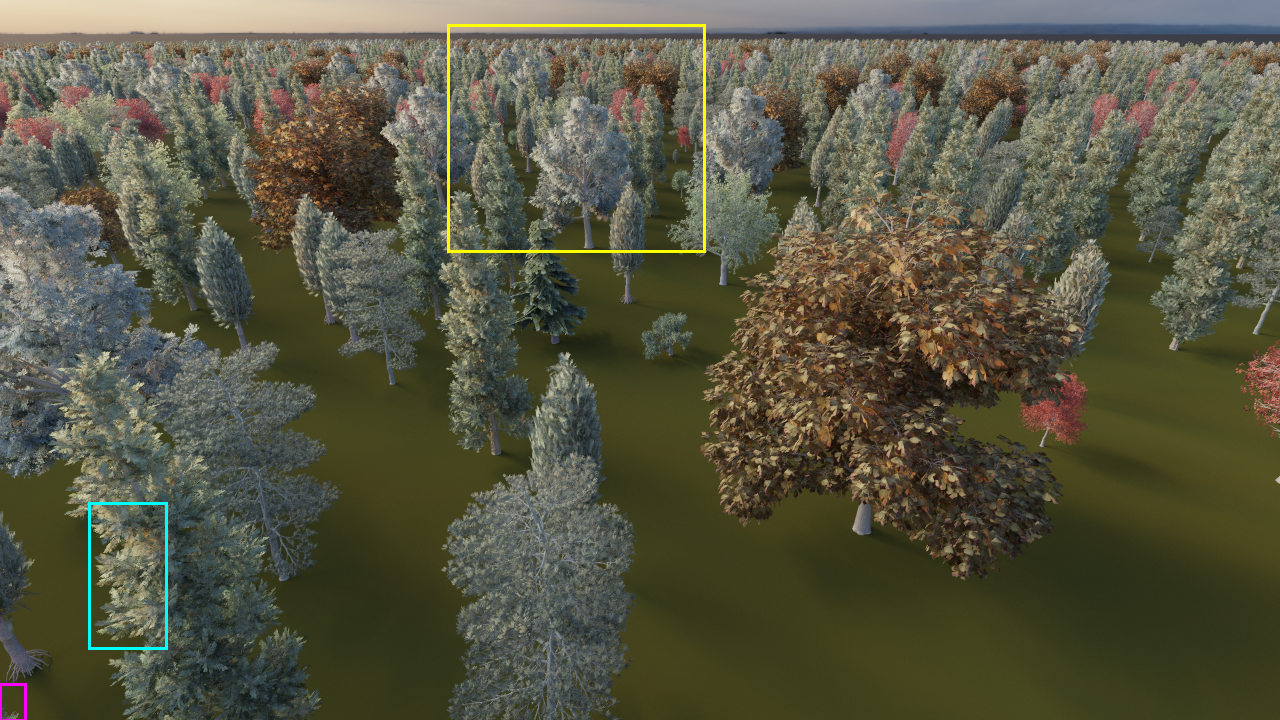
\includegraphics[height=4cm]{img/results/reference_with_boxes.png}%
            \quad
            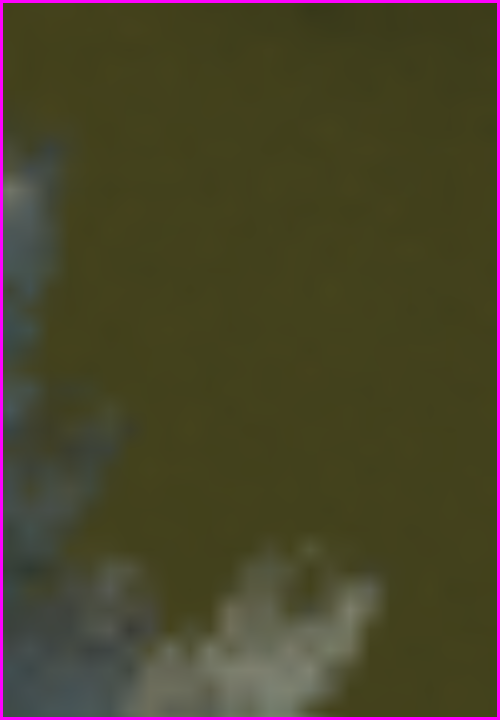
\includegraphics[height=4cm]{img/results/reference_snippet3.png}%
            \quad
            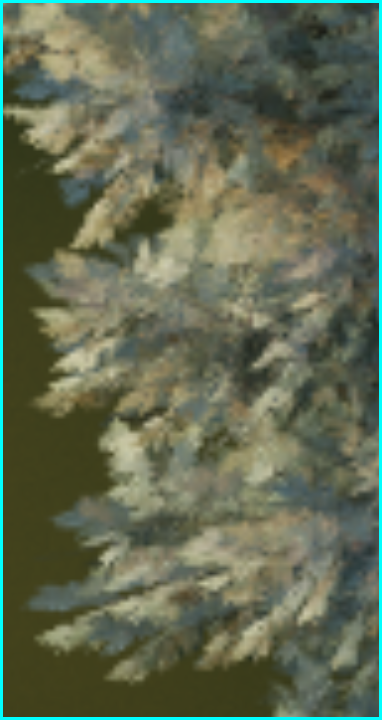
\includegraphics[height=4cm]{img/results/reference_snippet1.png}%
            \quad
            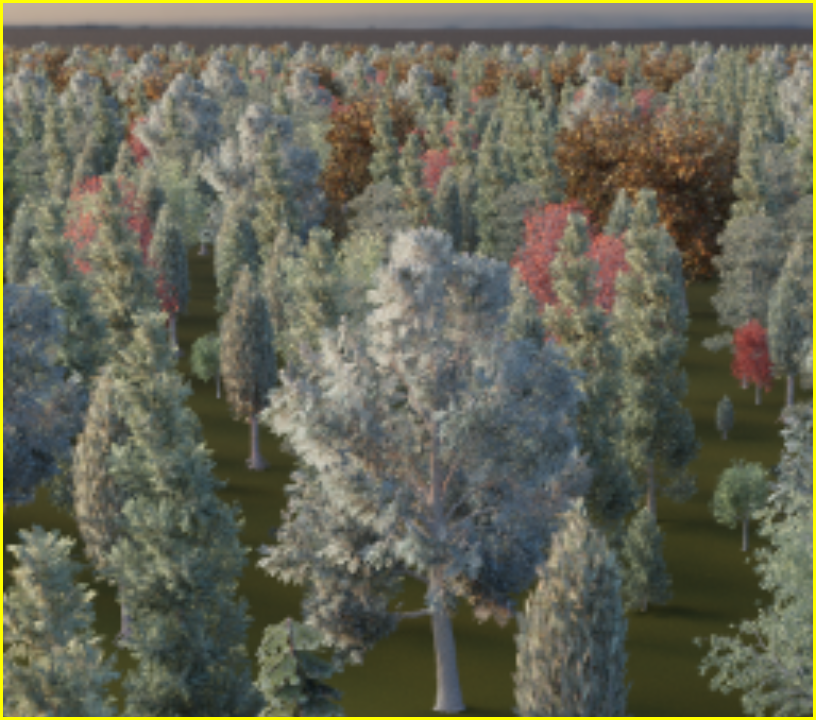
\includegraphics[height=4cm]{img/results/reference_snippet2.png}%
        }
        \caption{}
        \label{fig:render_comparison_mesh}
    \end{subfigure}
    \begin{subfigure}[b]{\linewidth}
        \resizebox{\textwidth}{!}{%
            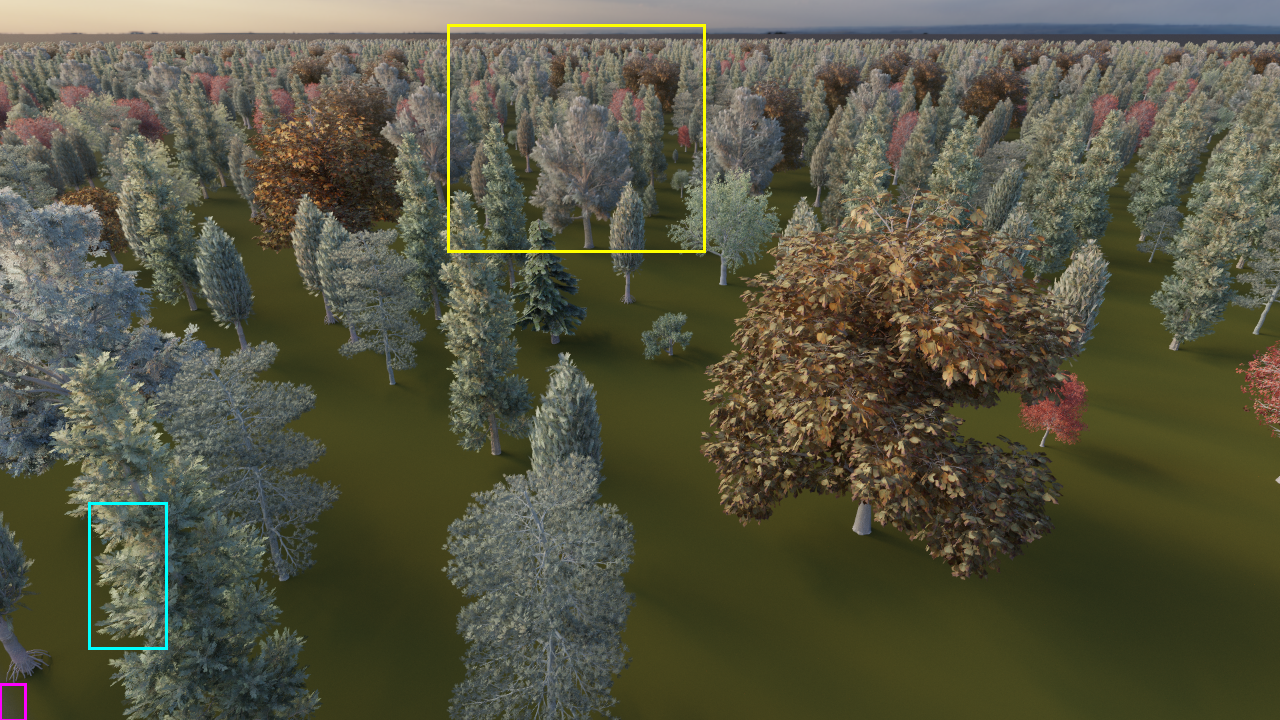
\includegraphics[height=4cm]{img/results/lod_1A_with_boxes.png}%
            \quad
            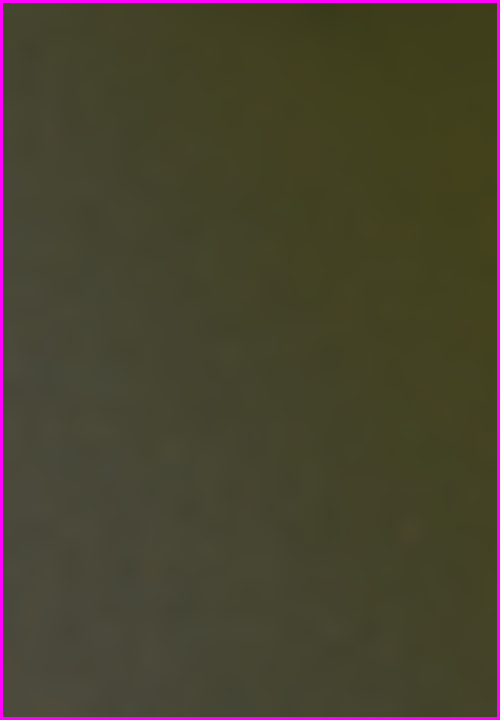
\includegraphics[height=4cm]{img/results/lod_1A_snippet3.png}%
            \quad
            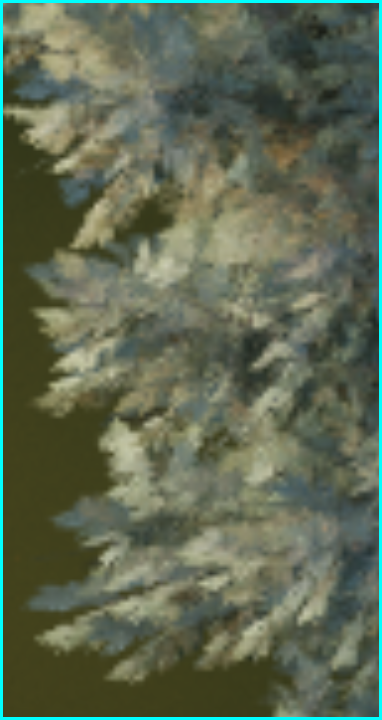
\includegraphics[height=4cm]{img/results/lod_1A_snippet1.png}%
            \quad
            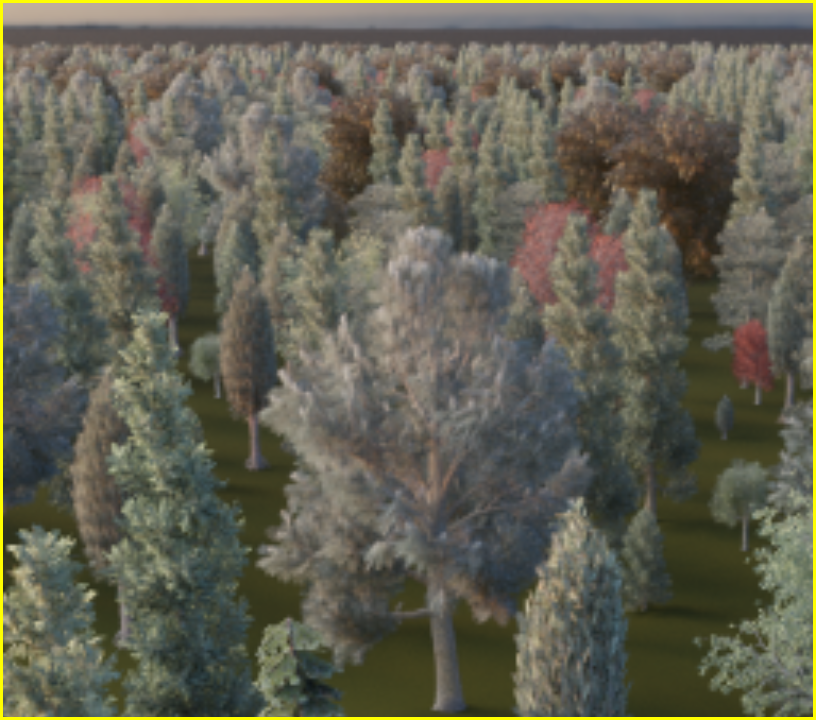
\includegraphics[height=4cm]{img/results/lod_1A_snippet2.png}%
        }
        \caption{}
        \label{fig:render_comparison_lod}
    \end{subfigure}
	\caption[Comparison between mesh and volume renderings of the forest]{(a) is the reference image rendered in $\SI{5463}{\s}$ with 1024 samples per pixel using only mesh representations, (b) uses \acsp{lod} if a voxel is smaller than a pixel and took $\SI{8723}{\s}$ to render with 1024 samples per pixel.}
	\label{fig:render_comparison}
\end{figure}
It can be observed, that the structure respectively the details of the \acs{lod} trees cannot be distinguished from the mesh representations which speaks for our heuristic for \ac{lod} selection.
However, when we look at the yellow framed image segment we see that the shading differs between both representations.
The volumetric trees generally look darker, which is especially pronounced on the side that faces the sun.
In the magenta framed image segment we can additionally see that a mesh is replaced by a volume, although it is clearly too close to the camera for the regular distance dependent \ac{lod} selection.
This is quite literally an edge case of our \ac{lod} selection procedure: We only check whether the vertices of the volumetric bounding box are within the view frustum, the edges connecting the vertices can still be visible in the frustum, thus making also the volume visible.
Unfortunately, we did not catch this shortcoming during development.
The differences in the cyan framed image segment are quite subtle: The tree in the reference rendering has a slight yellow tint that the \ac{lod} rendering lacks.
It is easier to see this error if we look at the \FLIP error map between the renderings in Figure \ref{fig:error_map}.
\begin{figure}[ht]
    \centering
    \resizebox{\textwidth}{!}{%
    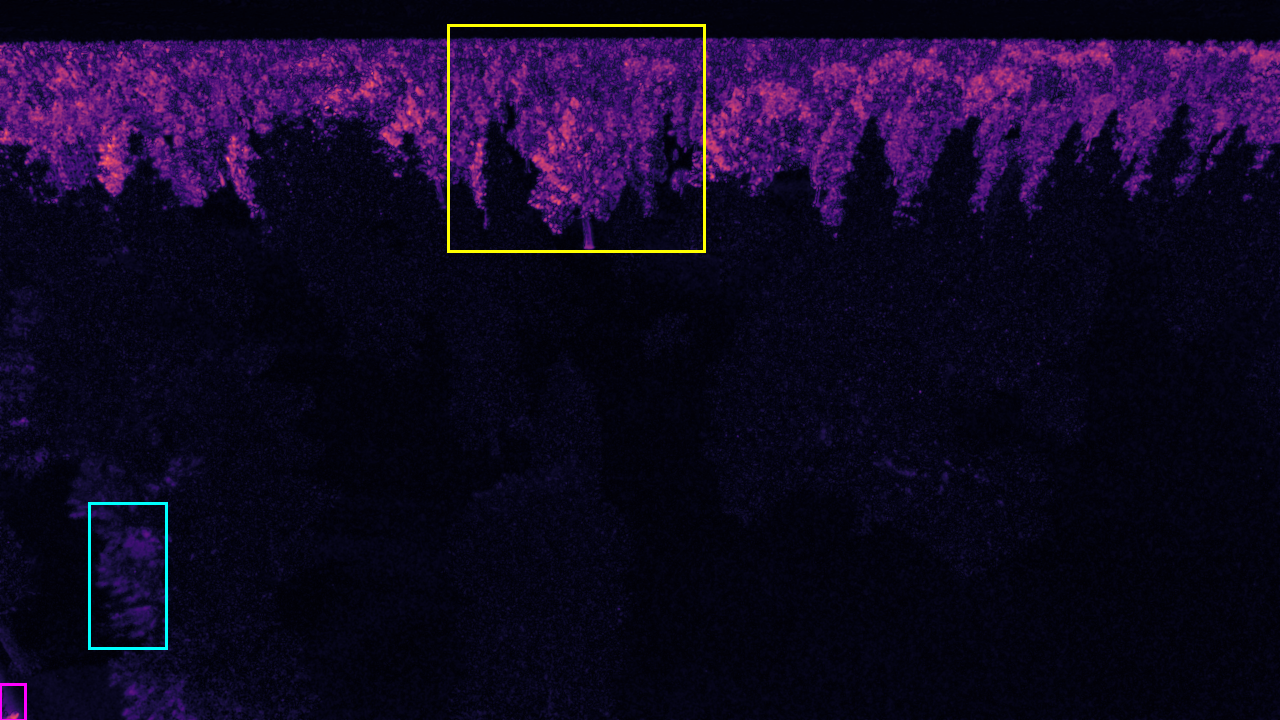
\includegraphics[height=4cm]{img/results/flip_error_1A_with_boxes.png}%
    \quad
    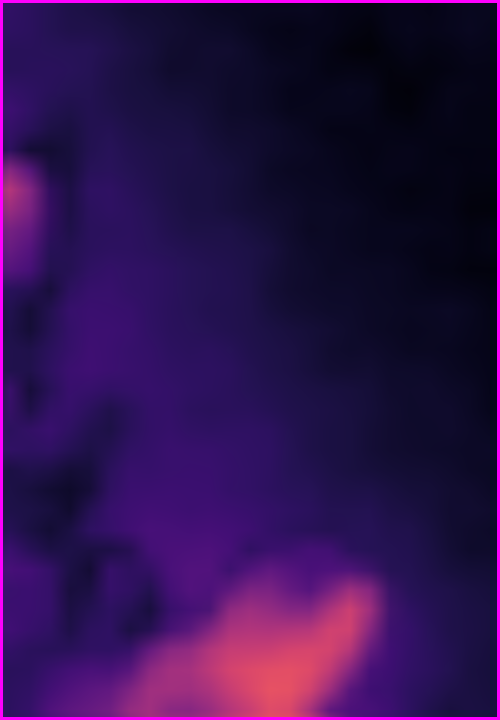
\includegraphics[height=4cm]{img/results/flip_error_1A_snippet3.png}%
    \quad
    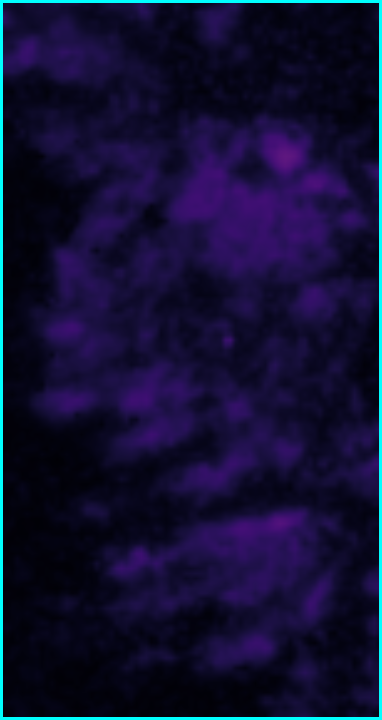
\includegraphics[height=4cm]{img/results/flip_error_1A_snippet1.png}%
    \quad
    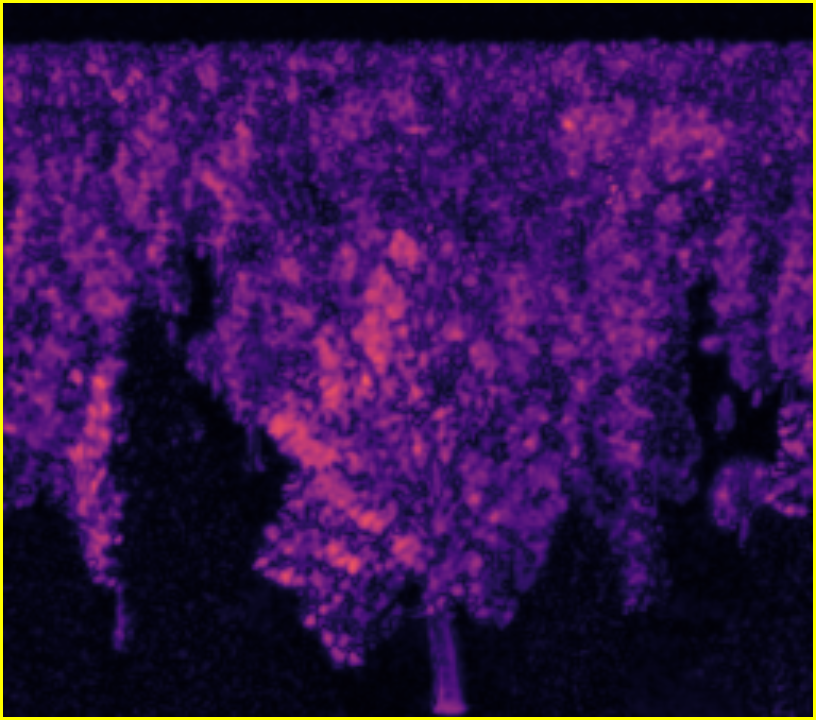
\includegraphics[height=4cm]{img/results/flip_error_1A_snippet2.png}%
    }
	\caption[\FLIP error map between reference and default \ac{lod} heuristic]{\FLIP error map between the reference rendering and the rendering using \acsp{lod} from Figure \ref{fig:render_comparison}. Dark regions indicate a low error, while bright regions indicate a high error. The mean \FLIP error is 0.073.}
	\label{fig:error_map}
\end{figure}
The tree in the cyan framed image segment visibly has an increased error compared to the surrounding trees.
This error is the result of indirect illumination: In the reference rendering there are mesh models outside the view frustum which reflect light on models in the view frustum.
These meshes outside the view frustum are replaced by volumes in the \ac{lod} rendering, which reflect less light.
The error map also makes the switch from mesh to volume rendering clearly visible, since the error suddenly increases.
As we observed in the renderings, the error is particularly high on the side that faces the sun.

In order to find the reason for the large shading difference on the sun-facing side, we split up the \acsp{brdf} and phase functions into the specular and diffuse component.
Intuitively we expect that these differences are specular highlights on the surfaces that are not rendered in the volumes.
However, looking at individual renderings of the diffuse and specular components in Figure \ref{fig:diffuse_specular_breakdown}, we find that these bright regions are in fact a result of the diffuse \ac{brdf}.
\begin{figure}[ht]
    \centering
    \begin{subfigure}[b]{0.49\linewidth}
        \centering
        \includegraphics[width=1\linewidth]{img/results/diffuse_only_mesh.jpg}
        \caption{}
        % \label{fig:render_comparison_mesh}
    \end{subfigure}
    \begin{subfigure}[b]{0.49\linewidth}
        \centering
        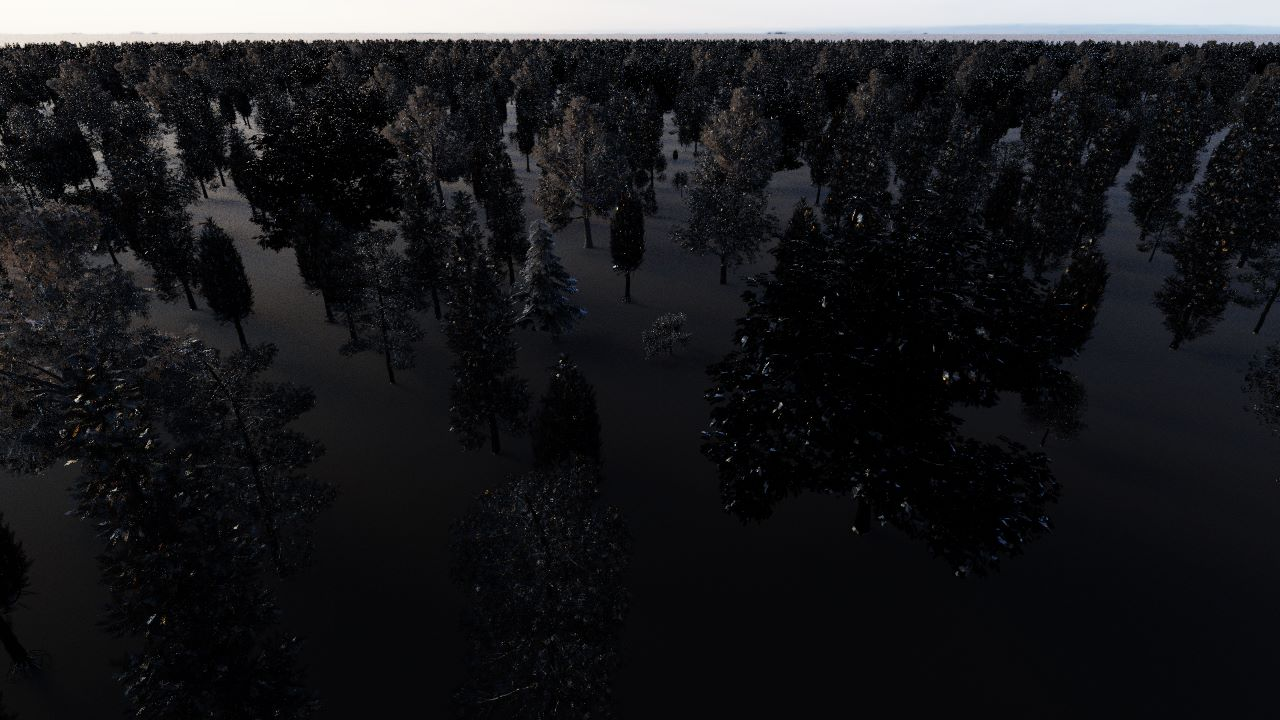
\includegraphics[width=1\linewidth]{img/results/specular_only_mesh.jpg}
        \caption{}
        % \label{fig:render_comparison_lod}
    \end{subfigure}
    \begin{subfigure}[b]{0.49\linewidth}
        \centering
        \includegraphics[width=1\linewidth]{img/results/diffuse_only_lod_1A.jpg}
        \caption{}
        % \label{fig:render_comparison_mesh}
    \end{subfigure}
    \begin{subfigure}[b]{0.49\linewidth}
        \centering
        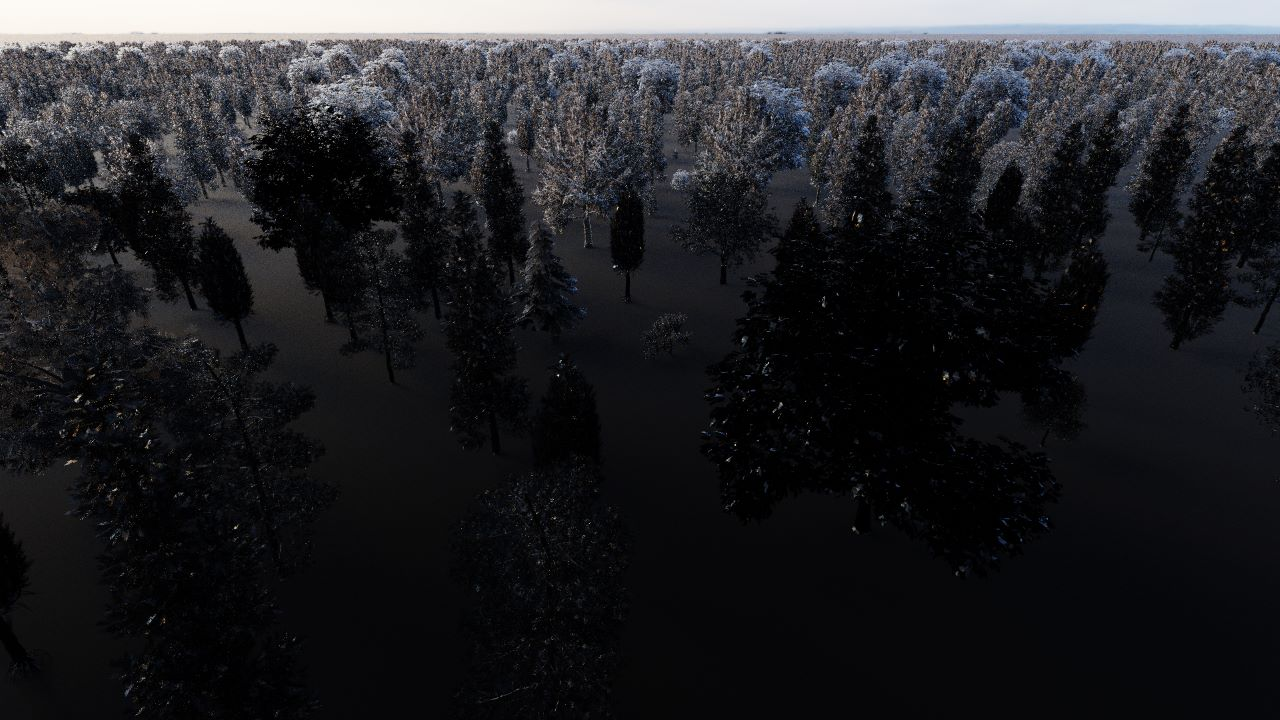
\includegraphics[width=1\linewidth]{img/results/specular_only_lod_1A.jpg}
        \caption{}
        % \label{fig:render_comparison_lod}
    \end{subfigure}
    % \caption[Comparison between mesh and volume renderings of the forest]{Renderings of the forest using meshes only (a) and using \acsp{lod} if a voxel is smaller than a pixel (b).}
    \caption[Diffuse and specular components rendered seperately]{(a) and (b) show the diffuse respectively specular component of the reference image, (c) and (d) show the diffuse respectively specular component when using \acsp{lod} where a voxel covers at most one pixel. The images are rendered with 32 samples per pixel.}
	\label{fig:diffuse_specular_breakdown}
\end{figure}
In the volumes, the diffuse phase function gives way more uniform looking trees without these bright regions on the sun-facing side.
The specular component gives discrete specular highlights on the surfaces while the specular phase function leads to reflections across the whole medium.
So our approach fails in preserving the visual appearance of the meshes.
We identify two reasons for this limitation: First, the \ac{sggx} phase function is defined on the whole unit sphere (recall Figure \ref{fig:sggx_ndf}), which means that half of the rays are reflected into the medium where they are attenuated, while for surfaces all rays are reflected away from the surface.
Second, it is likely that this error occured due to the usage of an isotropic microflake projected area, which directly influences our density values.
As we showed in Section \ref{sec:mesh_filtering} the optimization of the density depends on this projected area and by choosing a constant value we ignore for example how the roughness of a material influences the density, which would normally be reflected in the matrix $S$.
Using an anisotropic projected area therefore can lead to a significantly different look.
The filtering procedure however, would become more complex.
Experiments in this direction are outside of the scope of this thesis.

% This affects our density values, since the density is also optimized based on the microflake projected area $sigma$.
%  which effectively leads to reflection directions that are uniformly scattered on the unit sphere.
% % Second, it is likely that this error is due to the usage of an isotropic extinction coefficient, which effectively leads to reflection directions that are uniformly scattered on the unit sphere.
% Therefore we could reduce the error by using an anisotropic extinction, which would lead to a more complex filtering procedure.

Apart from these visual problems, the render time for the \ac{lod} approach is another concern.
The duration with $\SI{8723}{\s}$ for 1024 samples per pixel (Figure \ref{fig:render_comparison_lod}) is currently slower than rendering only the meshes, which took $\SI{5463}{\s}$ for 1024 samples per pixel (Figure \ref{fig:render_comparison_mesh}).
As we just discussed, we recognize the \acsp{lod} mainly by their different color and not by their details or blurriness.
We therefore have some room left for tweaking the distance at which we switch to \ac{lod} rendering or we can use coarser \acsp{lod}.
Tweaking the distance translates to changing the number of pixels a voxel may cover.
As we wrote in Section \ref{sec:scene_generation}, our heuristic currently ensures that a voxel covers at most one pixel.
Now we relax this restriction and measure render times when a voxel covers 1, 4, 9 or 16 pixels.
Additionally, we test how changing the voxel size of the finest \ac{lod} affects the performance.
In the first experiment, the voxels in our finest \ac{lod} had a size of 0.1m.
Now we choose a minimal voxel size of 0.1m, 0.2m, 0.4m, 0.8m, 1.6m, 3.2m and 6.4m.
In total this gives us 28 combinations that we have to test.
% We visualize our measurements in Figure \ref{fig:render_durations} as a heat map.
In Figure \ref{fig:lod_grid} we visualize the durations as well as the \FLIP error for rendering the different configurations with 32 samples per pixel.
\begin{figure}[ht]
    \centering
    \begin{subfigure}[b]{0.49\linewidth}
        \centering
        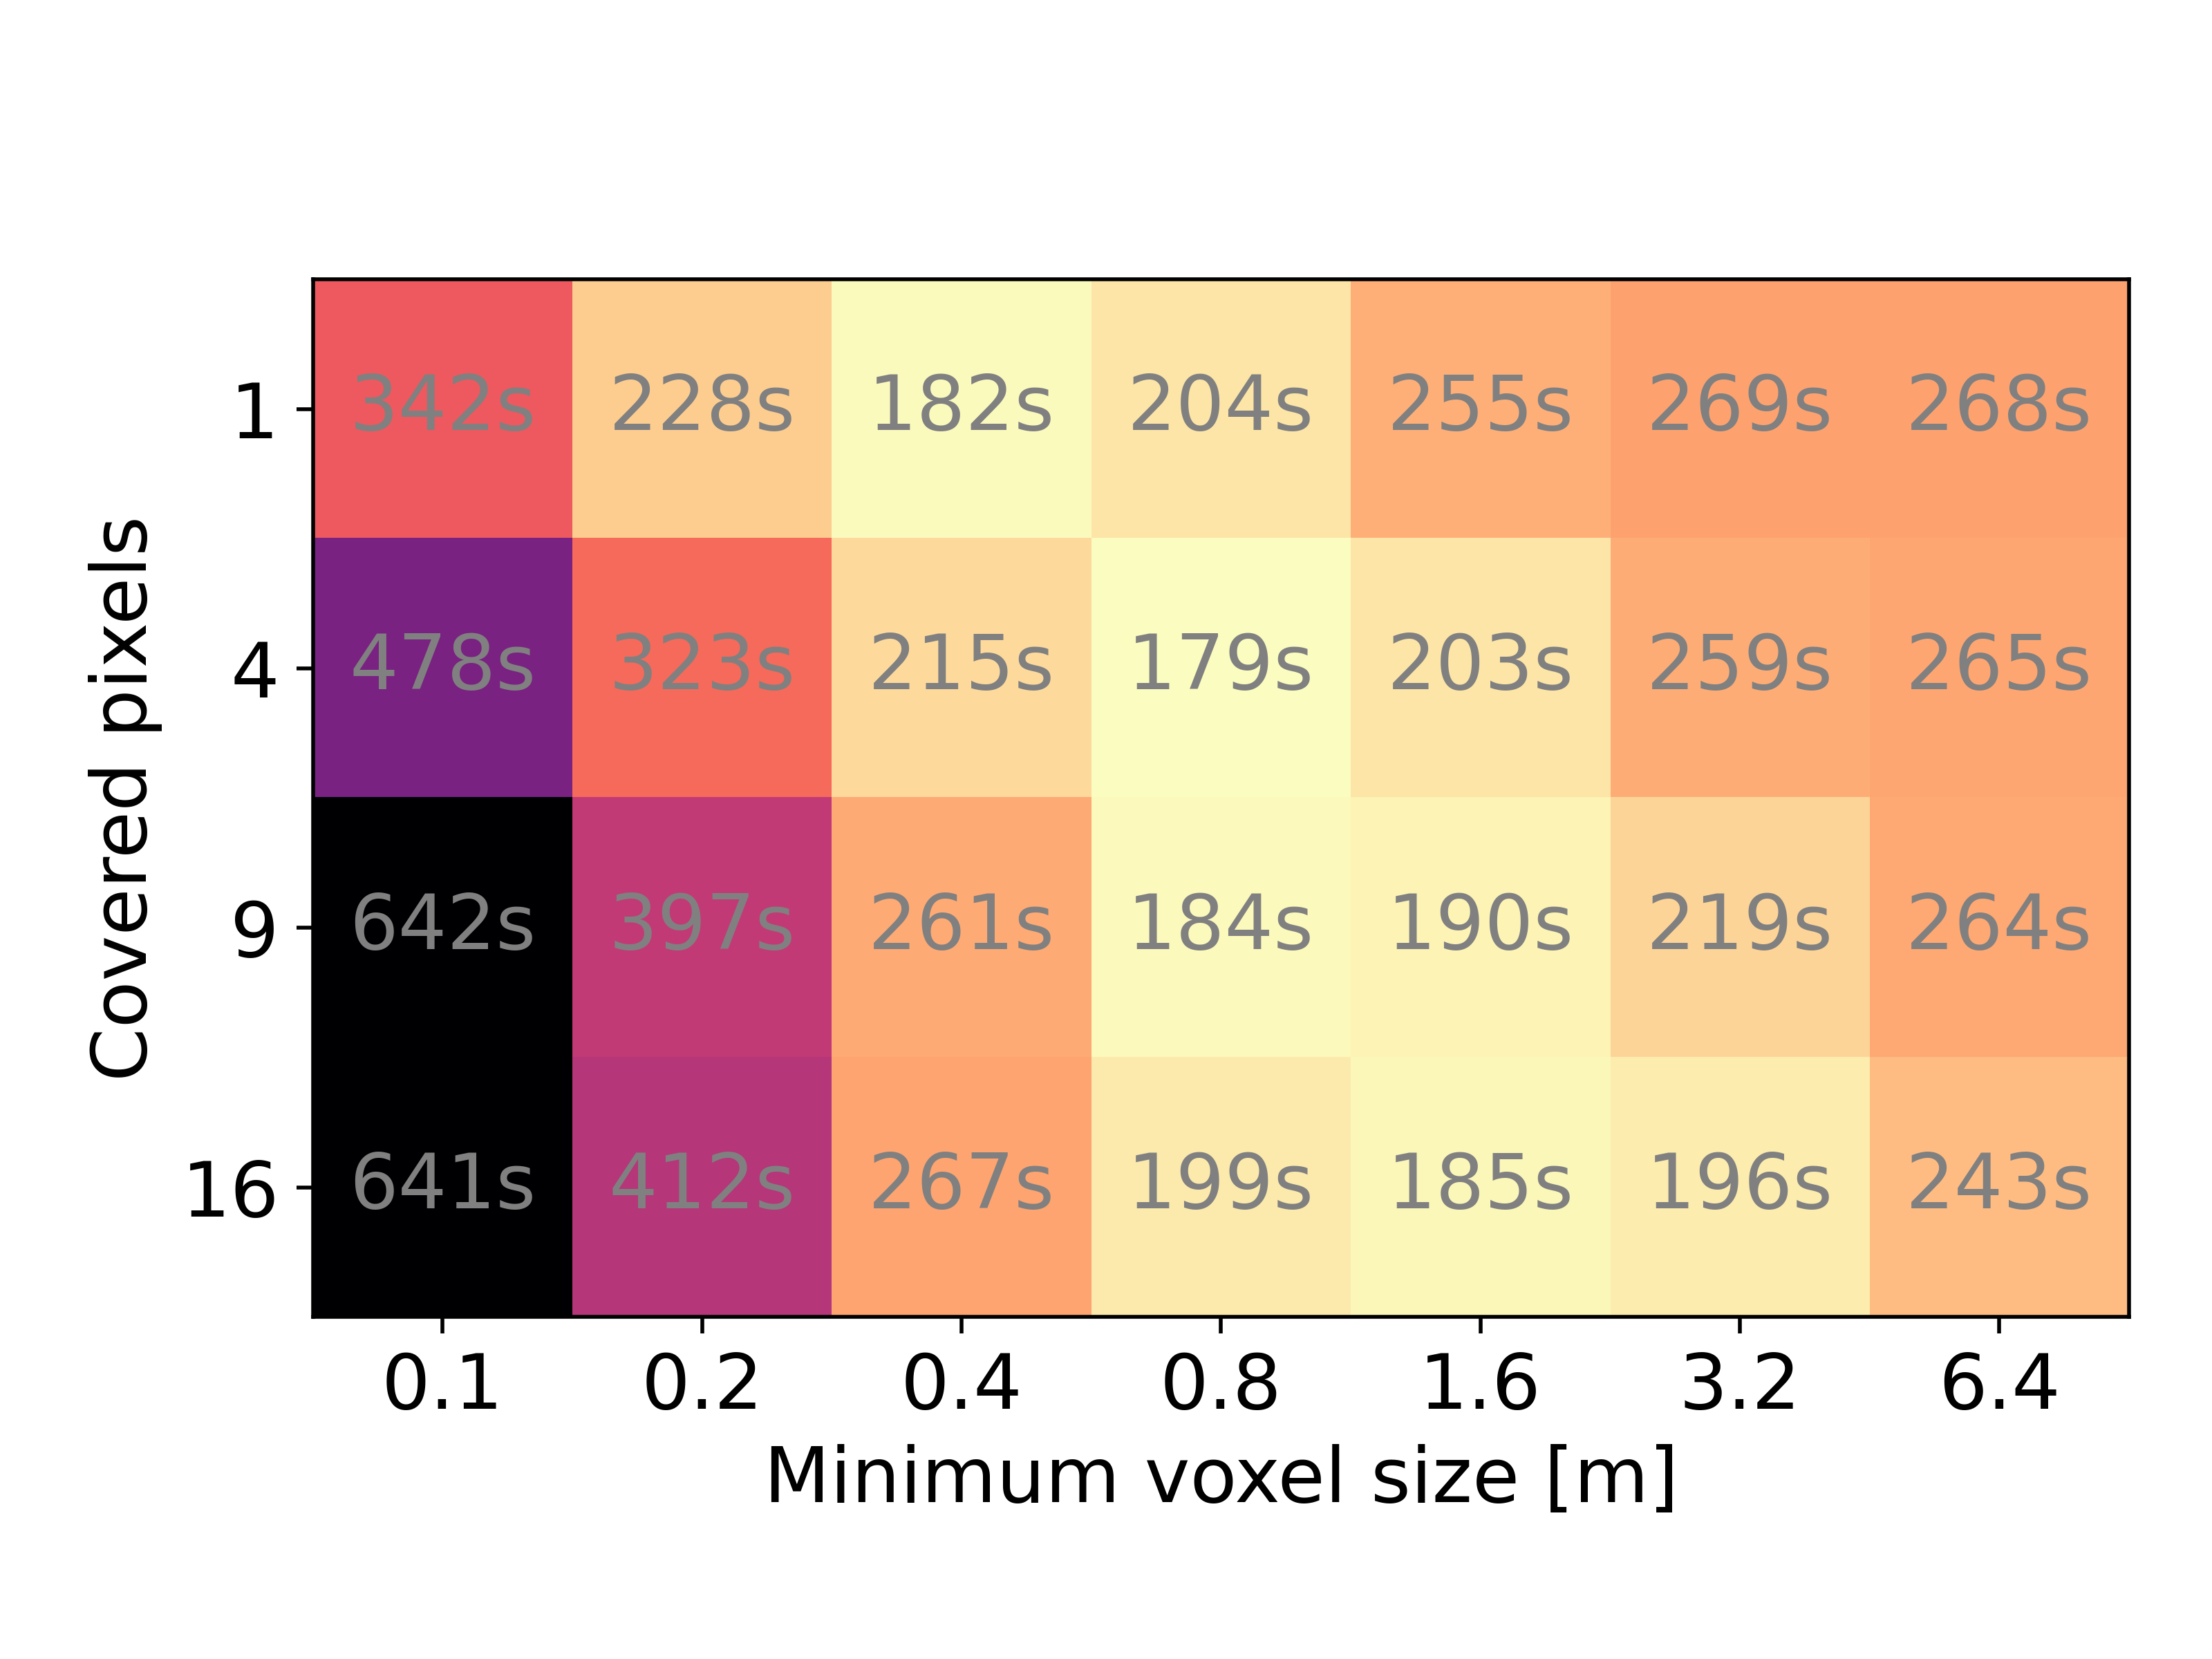
\includegraphics[width=1\linewidth]{img/results/render_durations.png}
        \caption{}
        \label{fig:lod_grid_durations}
    \end{subfigure}
    \begin{subfigure}[b]{0.49\linewidth}
        \centering
        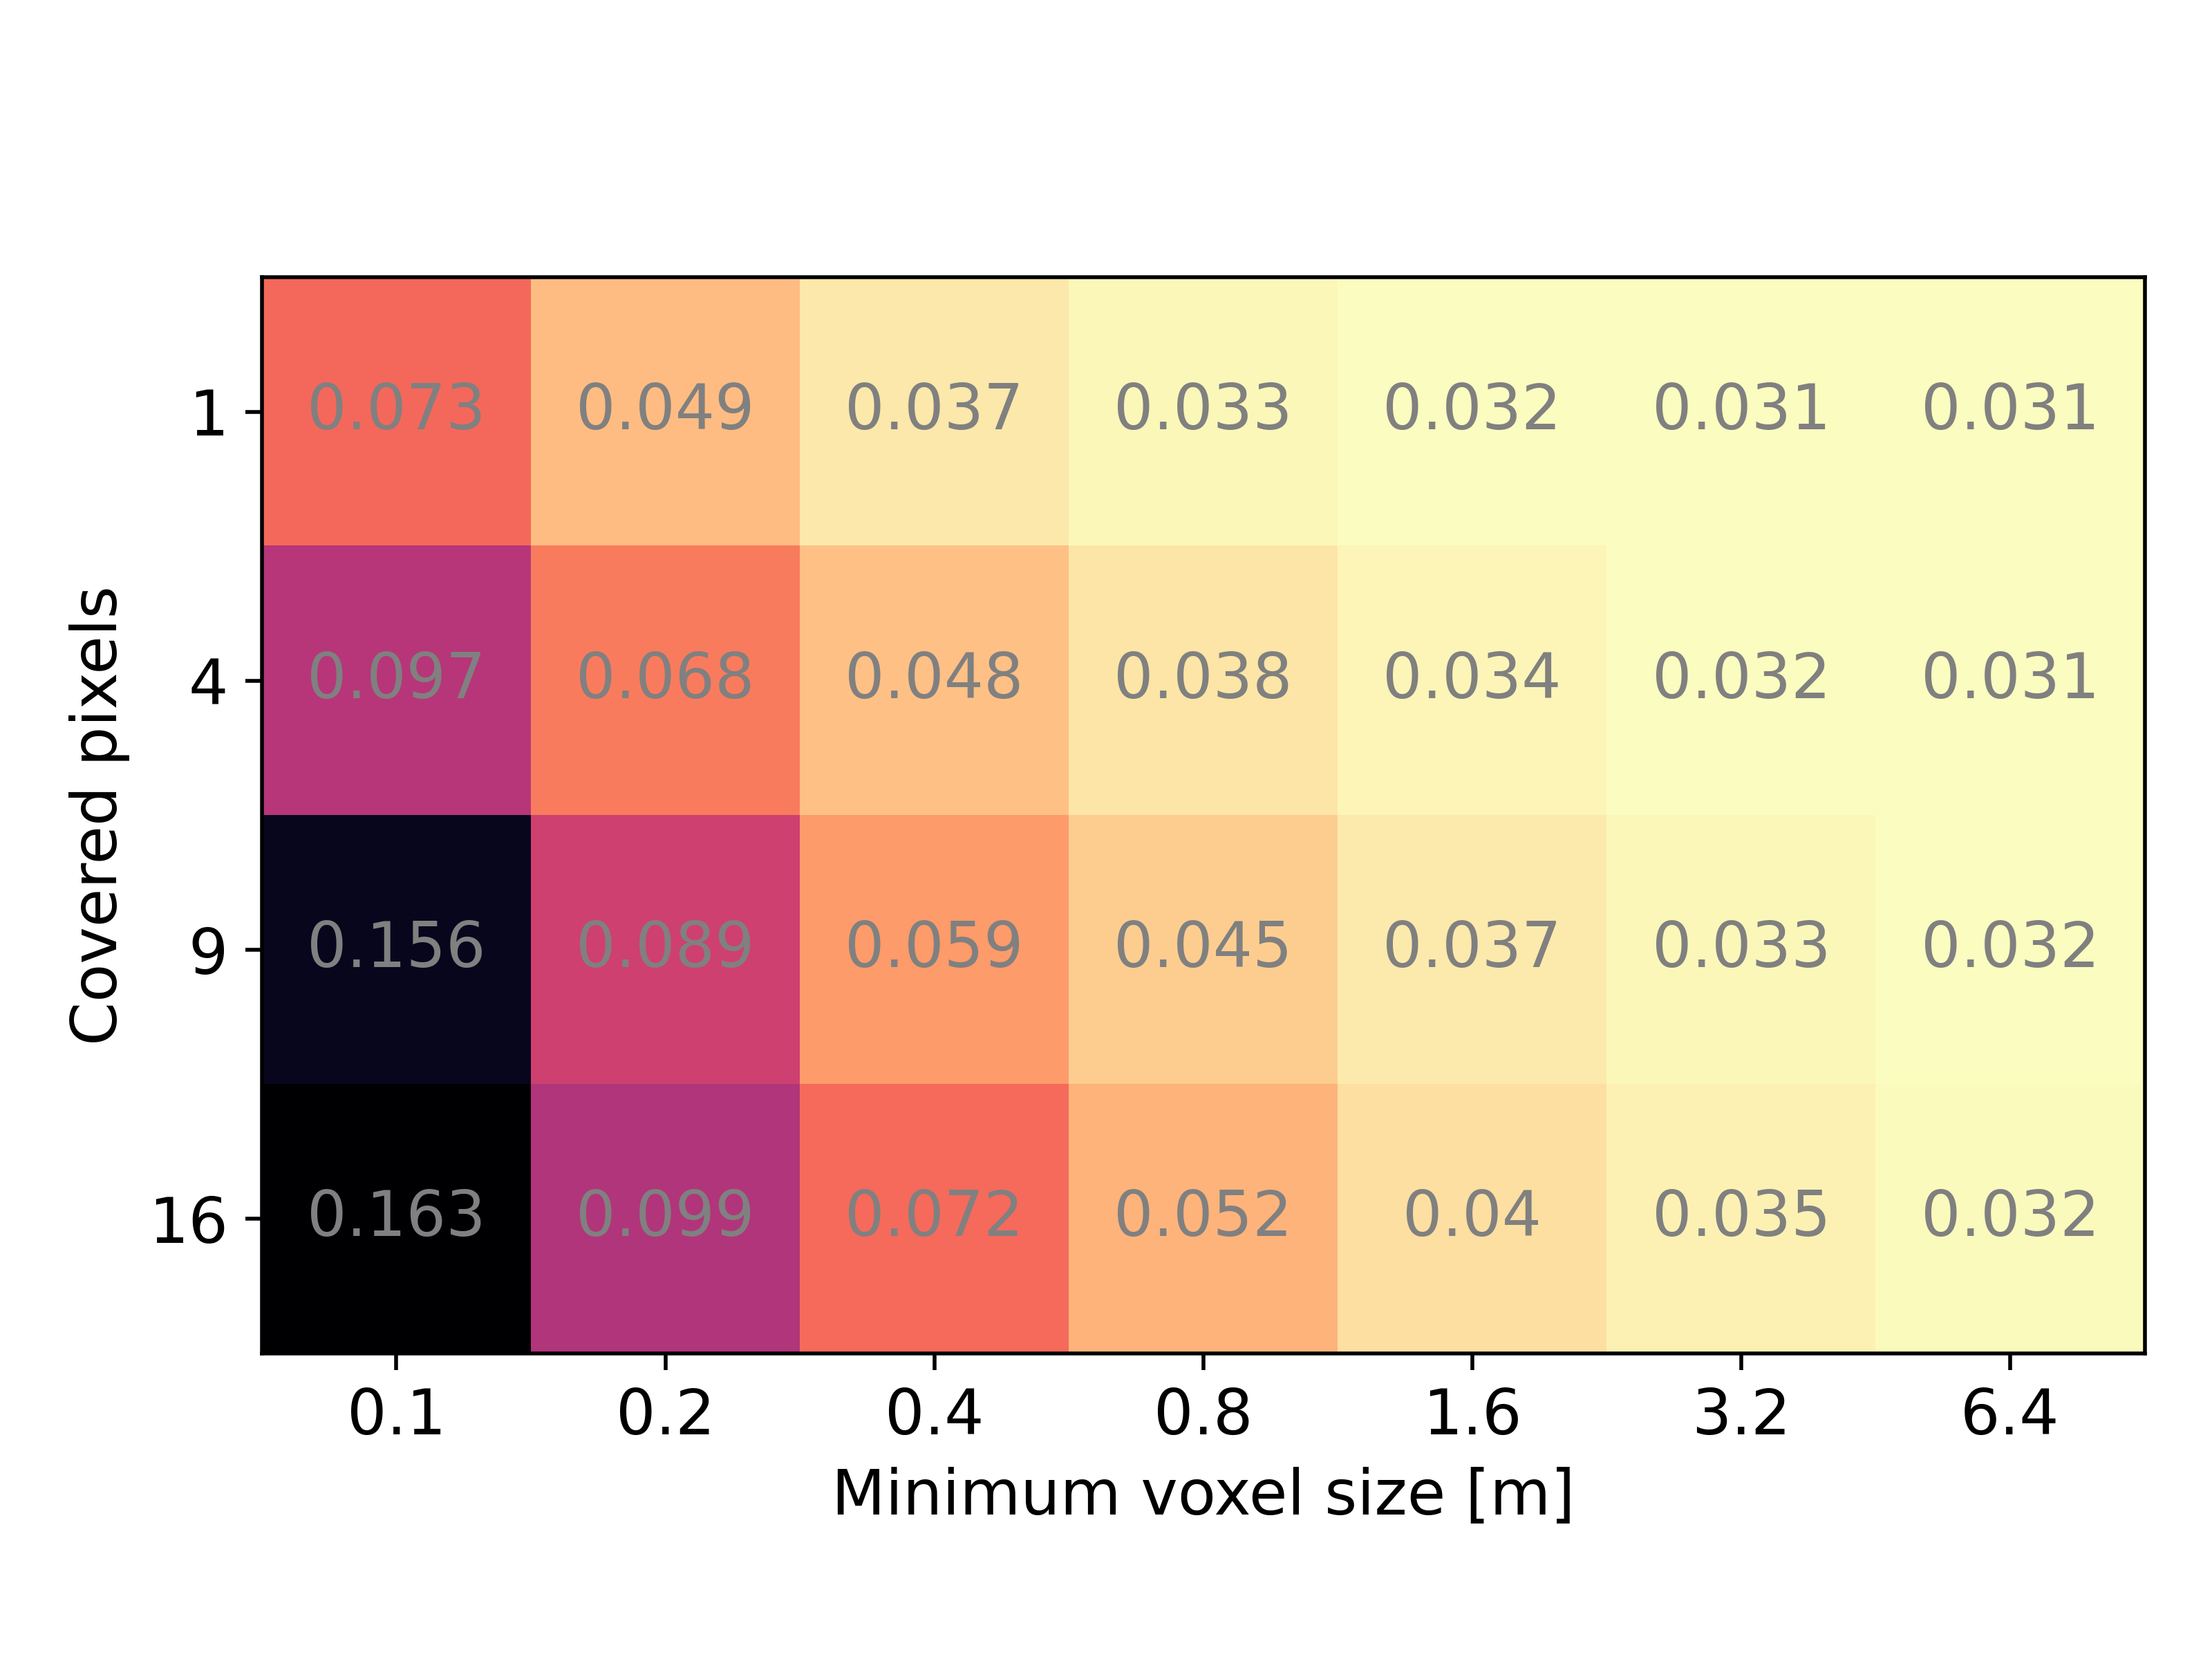
\includegraphics[width=1\linewidth]{img/results/flip_errors.png}
        \caption{}
    \end{subfigure}
	\caption[Heatmap of the \ac{lod} render durations and \FLIP errors]{Heatmap for render durations (a) and the mean \FLIP error (b) of different combinations of the minimum voxel size and the number of covered pixels. Bright regions indicate high values, dark regions indicate low values.}
	\label{fig:lod_grid}
\end{figure}
We can see that when we start \ac{lod} rendering with rougher \acsp{lod} we can reduce rendertimes to a certain degree before they rise again.
The decline happens because rougher \acsp{lod} are less memory intensive then the fine \acsp{lod} and therefore easier to cache.
At the same time increasing the minimum voxel size for a fixed number of covered pixels pushes the boundary of the \ac{lod} switch away from the camera which increases the number of meshes to be rendered.
The meshes take longer to render than the rough \acsp{lod}, therefore the render time increases again.

We get another view on the different combinations between the number of covered pixels and the minimum voxel size if we visualize the bounding boxes, like we previously did in Figure \ref{fig:visualize_lods}.
Now we not only show a rendering from above the scene but also from the main camera perspective.
Figure \ref{fig:visualize_lods_different_configurations_covered_pixels_fixed} visualizes the previously described effect, that the distance at which \acsp{lod} are rendered increases, when the minimum voxel size is increased.
\begin{figure}
    \begin{subfigure}[b]{\linewidth}
        \begin{center}
            \setlength{\tabcolsep}{2pt}
            \begin{tabular}{ c c c c  }
                \adjustimage{width=0.24\textwidth,valign=m}{img/results/visualize_lods_1A_front.jpg} & \adjustimage{width=0.24\textwidth,valign=m}{img/results/visualize_lods_1B_front.jpg} & \adjustimage{width=0.24\textwidth,valign=m}{img/results/visualize_lods_1C_front.jpg} & \adjustimage{width=0.24\textwidth,valign=m}{img/results/visualize_lods_1D_front.jpg} \\
                \adjustimage{width=0.24\textwidth,valign=m}{img/results/visualize_lods_1A_top.jpg} & \adjustimage{width=0.24\textwidth,valign=m}{img/results/visualize_lods_1B_top.jpg} & \adjustimage{width=0.24\textwidth,valign=m}{img/results/visualize_lods_1C_top.jpg} & \adjustimage{width=0.24\textwidth,valign=m}{img/results/visualize_lods_1D_top.jpg} \\
                {\footnotesize Covered pixels = 1} & {\footnotesize Covered pixels = 4} & {\footnotesize Covered pixels = 9} & {\footnotesize Covered pixels = 16} \\
            \end{tabular}
        \end{center}
        \caption{}
        \label{fig:visualize_lods_different_configurations_min_voxel_size_fixed}
    \end{subfigure}
    \begin{subfigure}[b]{\linewidth}
        \begin{center}
            \setlength{\tabcolsep}{2pt}
            \begin{tabular}{ c c c c  }
                \adjustimage{width=0.24\textwidth,valign=m}{img/results/visualize_lods_1A_front.jpg} & \adjustimage{width=0.24\textwidth,valign=m}{img/results/visualize_lods_2A_front.jpg} & \adjustimage{width=0.24\textwidth,valign=m}{img/results/visualize_lods_3A_front.jpg} & \adjustimage{width=0.24\textwidth,valign=m}{img/results/visualize_lods_4A_front.jpg} \\
                \adjustimage{width=0.24\textwidth,valign=m}{img/results/visualize_lods_1A_top.jpg} & \adjustimage{width=0.24\textwidth,valign=m}{img/results/visualize_lods_2A_top.jpg} & \adjustimage{width=0.24\textwidth,valign=m}{img/results/visualize_lods_3A_top.jpg} & \adjustimage{width=0.24\textwidth,valign=m}{img/results/visualize_lods_4A_top.jpg} \\
                % Covered pixels = 1 & Covered pixels = 4 & Covered pixels = 9 & Covered pixels = 16 \\
                {\footnotesize Min. voxel size = $\SI{0.1}{\m}$} & {\footnotesize Min. voxel size = $\SI{0.2}{\m}$} & {\footnotesize Min. voxel size = $\SI{0.4}{\m}$} & {\footnotesize Min.\newline voxel size = $\SI{0.8}{\m}$}\\
            \end{tabular}
        \end{center}
        \caption{}
        \label{fig:visualize_lods_different_configurations_covered_pixels_fixed}
    \end{subfigure}
    \caption[Visualization of \acsp{lod} using different configurations]{Debug views of the volume bounding boxes for different configurations. In (a) the minimum voxel size is fixed at $\SI{0.1}{\m}$ and we vary the number of covered pixels, while in (b) the number of covered pixels is fixed at 1 and we vary the minimum voxel size. Blue is again the finest \ac{lod} and red the coarsest \ac{lod}. }
    \label{fig:visualize_lods_different_configurations}
\end{figure}
For the case of a fixed number of covered pixels and a minimum voxel size of $\SI{0.8}{\m}$, it is also interesting to note that the distance based \acsp{lod} still cover almost half of the circular forest, although they are barely visible from the main camera's perspective.
Figure \ref{fig:visualize_lods_different_configurations_min_voxel_size_fixed} on the other hand, is analogous to the first column of Figure \ref{fig:lod_grid_durations} as we also fixed the minimum voxel size at $\SI{0.1}{\m}$ and increase the number of covered pixels.
The figure intuitively explains the near doubling of the render time between 1 covered pixel and 16 covered pixels, since we start \ac{lod} rendering right in front of the camera for 16 covered pixels.


% We get another view on the increasing distances of \ac{lod} rendering when we look at the colored bounding boxes of the volumes again ...
Looking back at Figure \ref{fig:lod_grid}, the overall best result is achieved by dropping the three finest \acsp{lod} and let each voxel cover up to four pixels.
The scene then renders in $\SI{4549}{\s}$ which is a 17\% improvement over rendering only meshes.
Additionally, it has the positive side-effect that the shading problem is less noticeable, which is reflected in a drop in the mean \FLIP error from 0.073 to 0.038.
Figure \ref{fig:render_and_error_fastest} shows this rendering with the corresponding \FLIP error map.
\begin{figure}[ht]
    \centering
    \begin{subfigure}[b]{\linewidth}
        \resizebox{\textwidth}{!}{%
            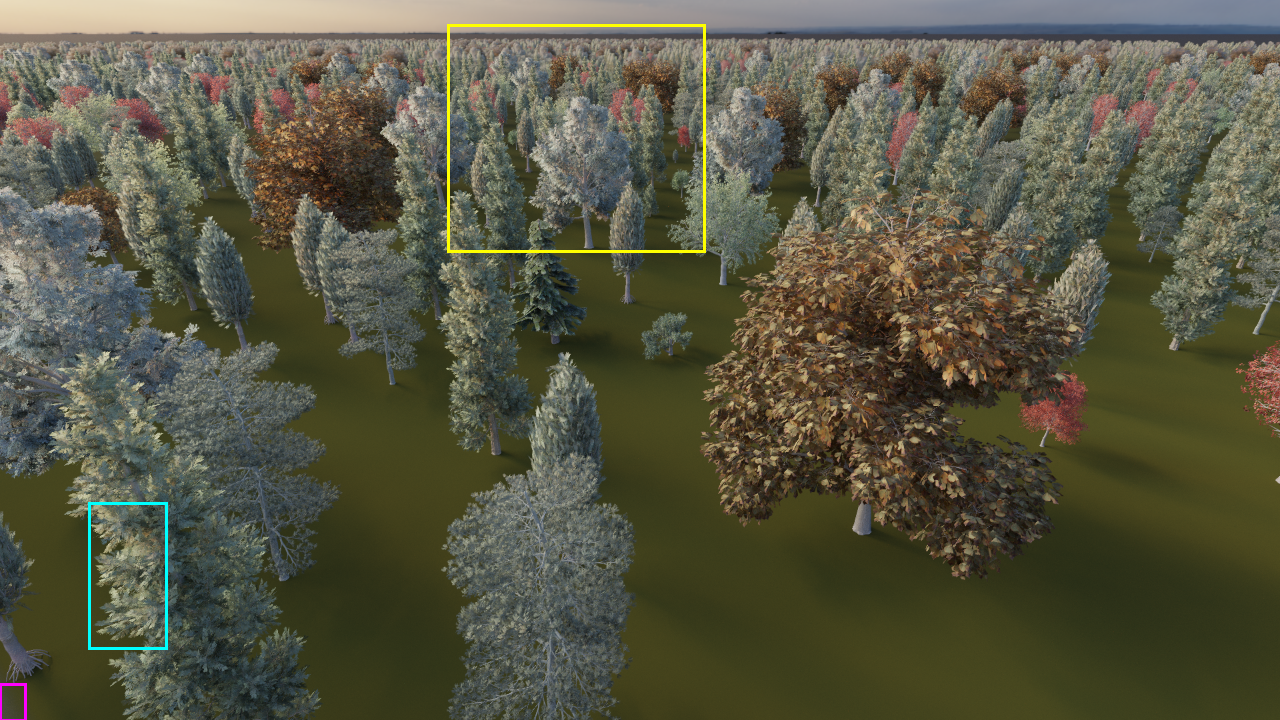
\includegraphics[height=4cm]{img/results/lod_4B_with_boxes.png}%
            \quad
            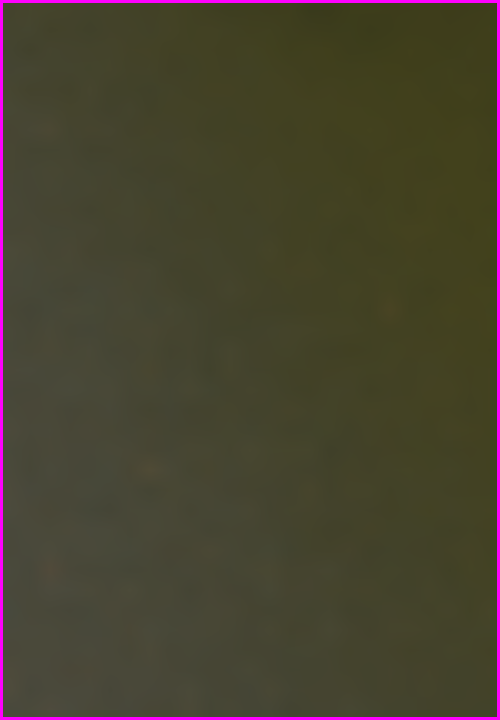
\includegraphics[height=4cm]{img/results/lod_4B_snippet3.png}%
            \quad
            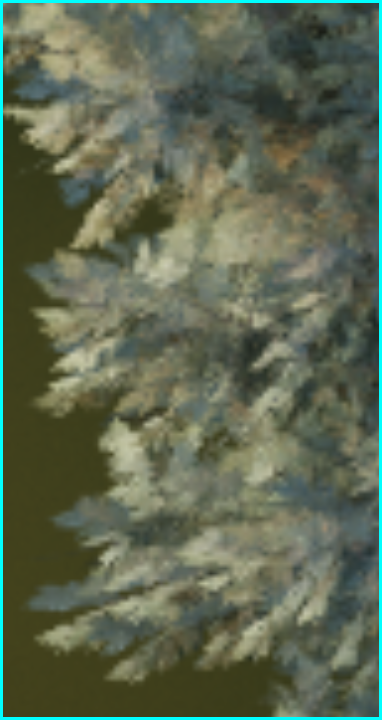
\includegraphics[height=4cm]{img/results/lod_4B_snippet1.png}%
            \quad
            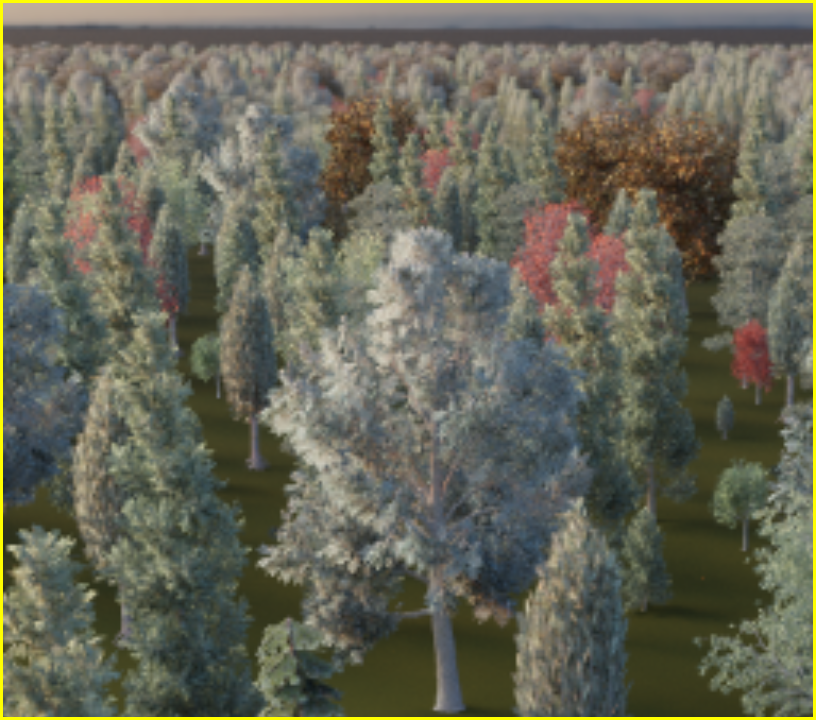
\includegraphics[height=4cm]{img/results/lod_4B_snippet2.png}%
        }
        \caption{}
    \end{subfigure}
    \begin{subfigure}[b]{\linewidth}
        \resizebox{\textwidth}{!}{%
            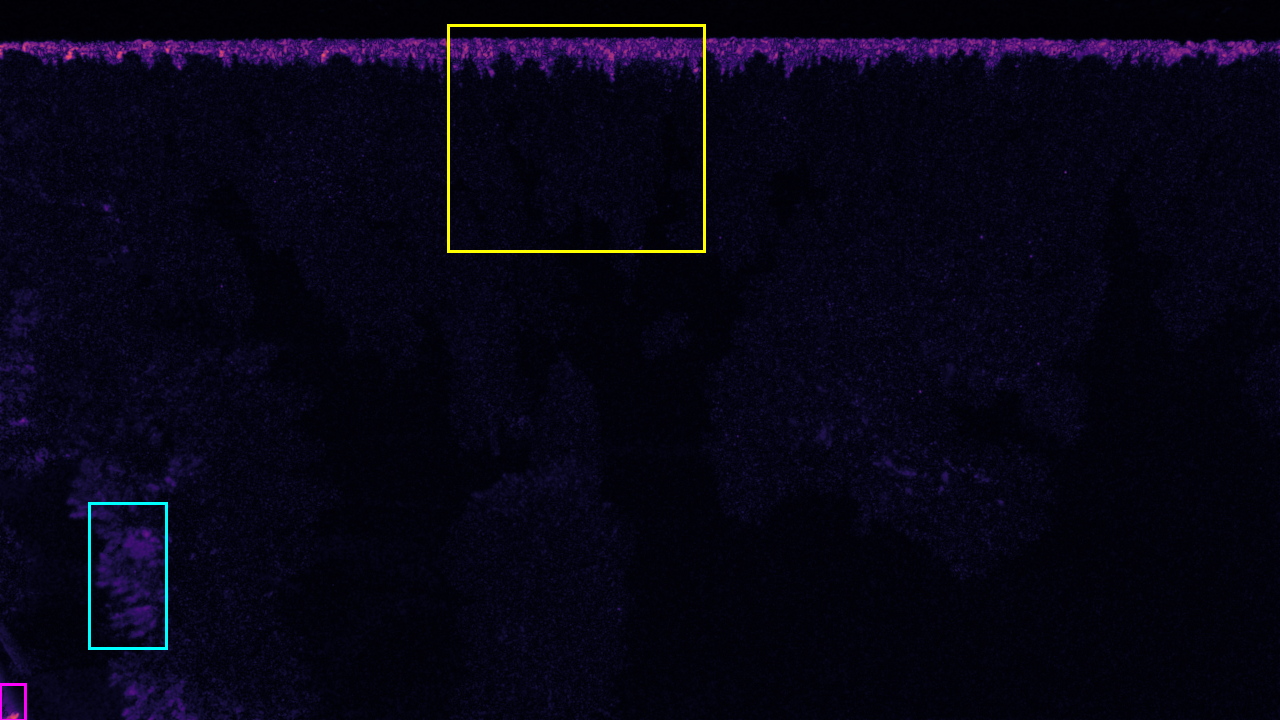
\includegraphics[height=4cm]{img/results/flip_error_4B_with_boxes.png}%
            \quad
            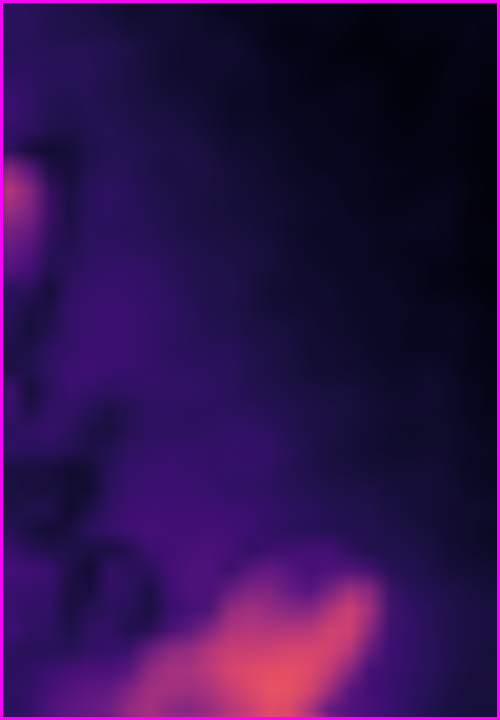
\includegraphics[height=4cm]{img/results/flip_error_4B_snippet3.png}%
            \quad
            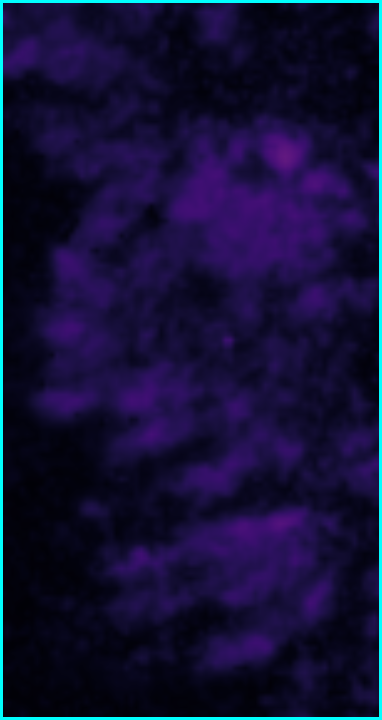
\includegraphics[height=4cm]{img/results/flip_error_4B_snippet1.png}%
            \quad
            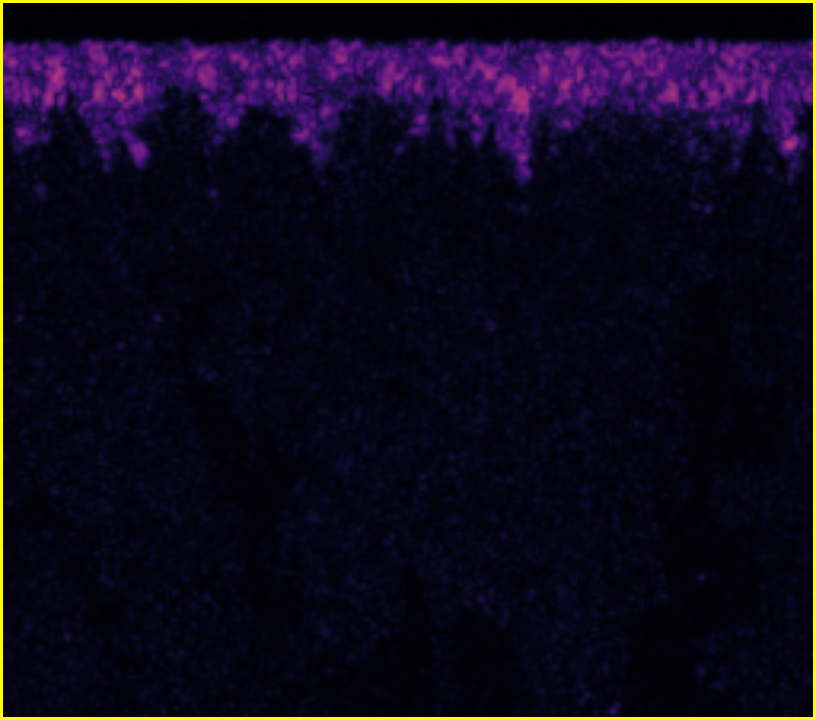
\includegraphics[height=4cm]{img/results/flip_error_4B_snippet2.png}%
        }
        \caption{}
    \end{subfigure}
    \caption[Rendering and \FLIP error map of the fastest combination]{(a) shows the fastest rendering, finished in $\SI{4548}{\s}$ for 1024 samples. The scene is generated with a minimum voxel size of 0.8m and up to four covered pixels per voxel. (b) shows the corresponding \FLIP error map against the ground truth. The mean \FLIP error is 0.038.}
    \label{fig:render_and_error_fastest}
\end{figure}
We can further decrease the mean \FLIP error down to 0.031, for example by choosing a minimum voxel size of 6.4 meters and let each voxel cover one pixel, at the cost of a higher render time.

\section{Experiments on Single Model Instances}
\label{sec:experiments_on_single_model_instances}
Now that we have a good idea of the performance and quality implications of our approach we perform further tests on single instances of some tree models.
This gives us finer control over which \ac{lod} should be rendered at which distance.
We use the models \textit{Celtis australis adult} (Figure \ref{fig:EU06a}) and \textit{Acer rubrum adult} (Figure \ref{fig:EA01a}) for our tests.
\begin{figure}[ht]
    \centering
    \begin{subfigure}[b]{0.49\linewidth}
        \centering
        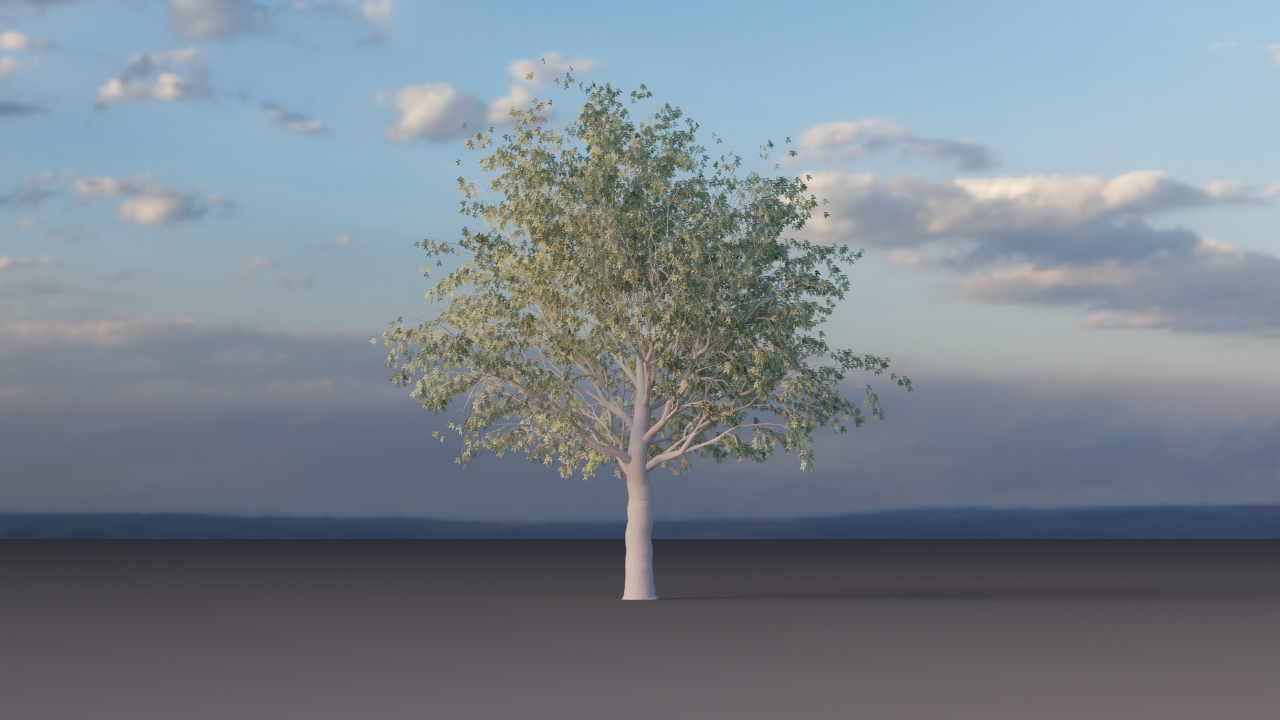
\includegraphics[width=1\linewidth]{img/results/EU06a.png}
        \caption{}
        \label{fig:EU06a}
    \end{subfigure}
    \begin{subfigure}[b]{0.49\linewidth}
        \centering
        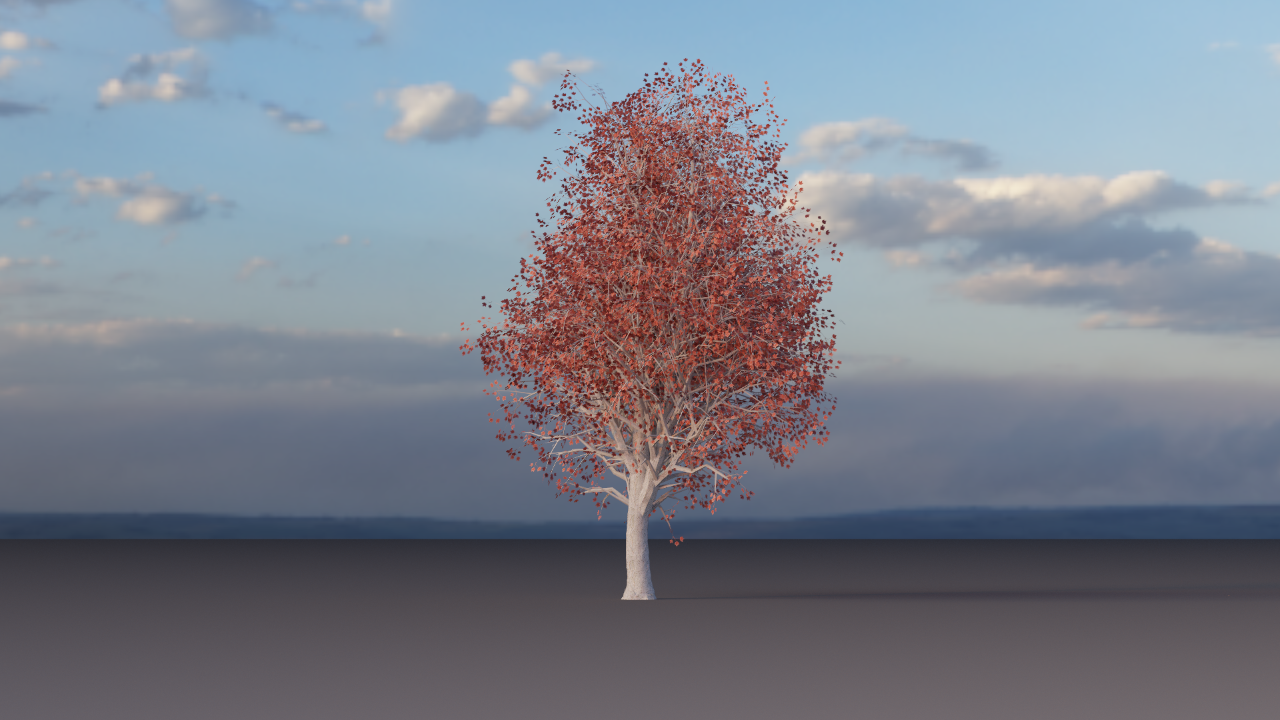
\includegraphics[width=1\linewidth]{img/results/EA01a.png}
        \caption{}
        \label{fig:EA01a}
    \end{subfigure}
	\caption[Models for single instance experiments]{We use the model \textit{Celtis australis adult} (a) and \textit{Acer rubrum adult} (b) for our single instance experiments. Both images show the mesh representations.}
	\label{fig:single_model_instances}
\end{figure}

The first experiment in this context is, that we render a single instance of all mesh and volume representations at different distances.
We can see the rendertimes of this experiment plotted in Figure \ref{fig:render_time_comparisons}.
\begin{figure}[ht]
    \centering
    \begin{subfigure}[b]{0.49\linewidth}
        \centering
        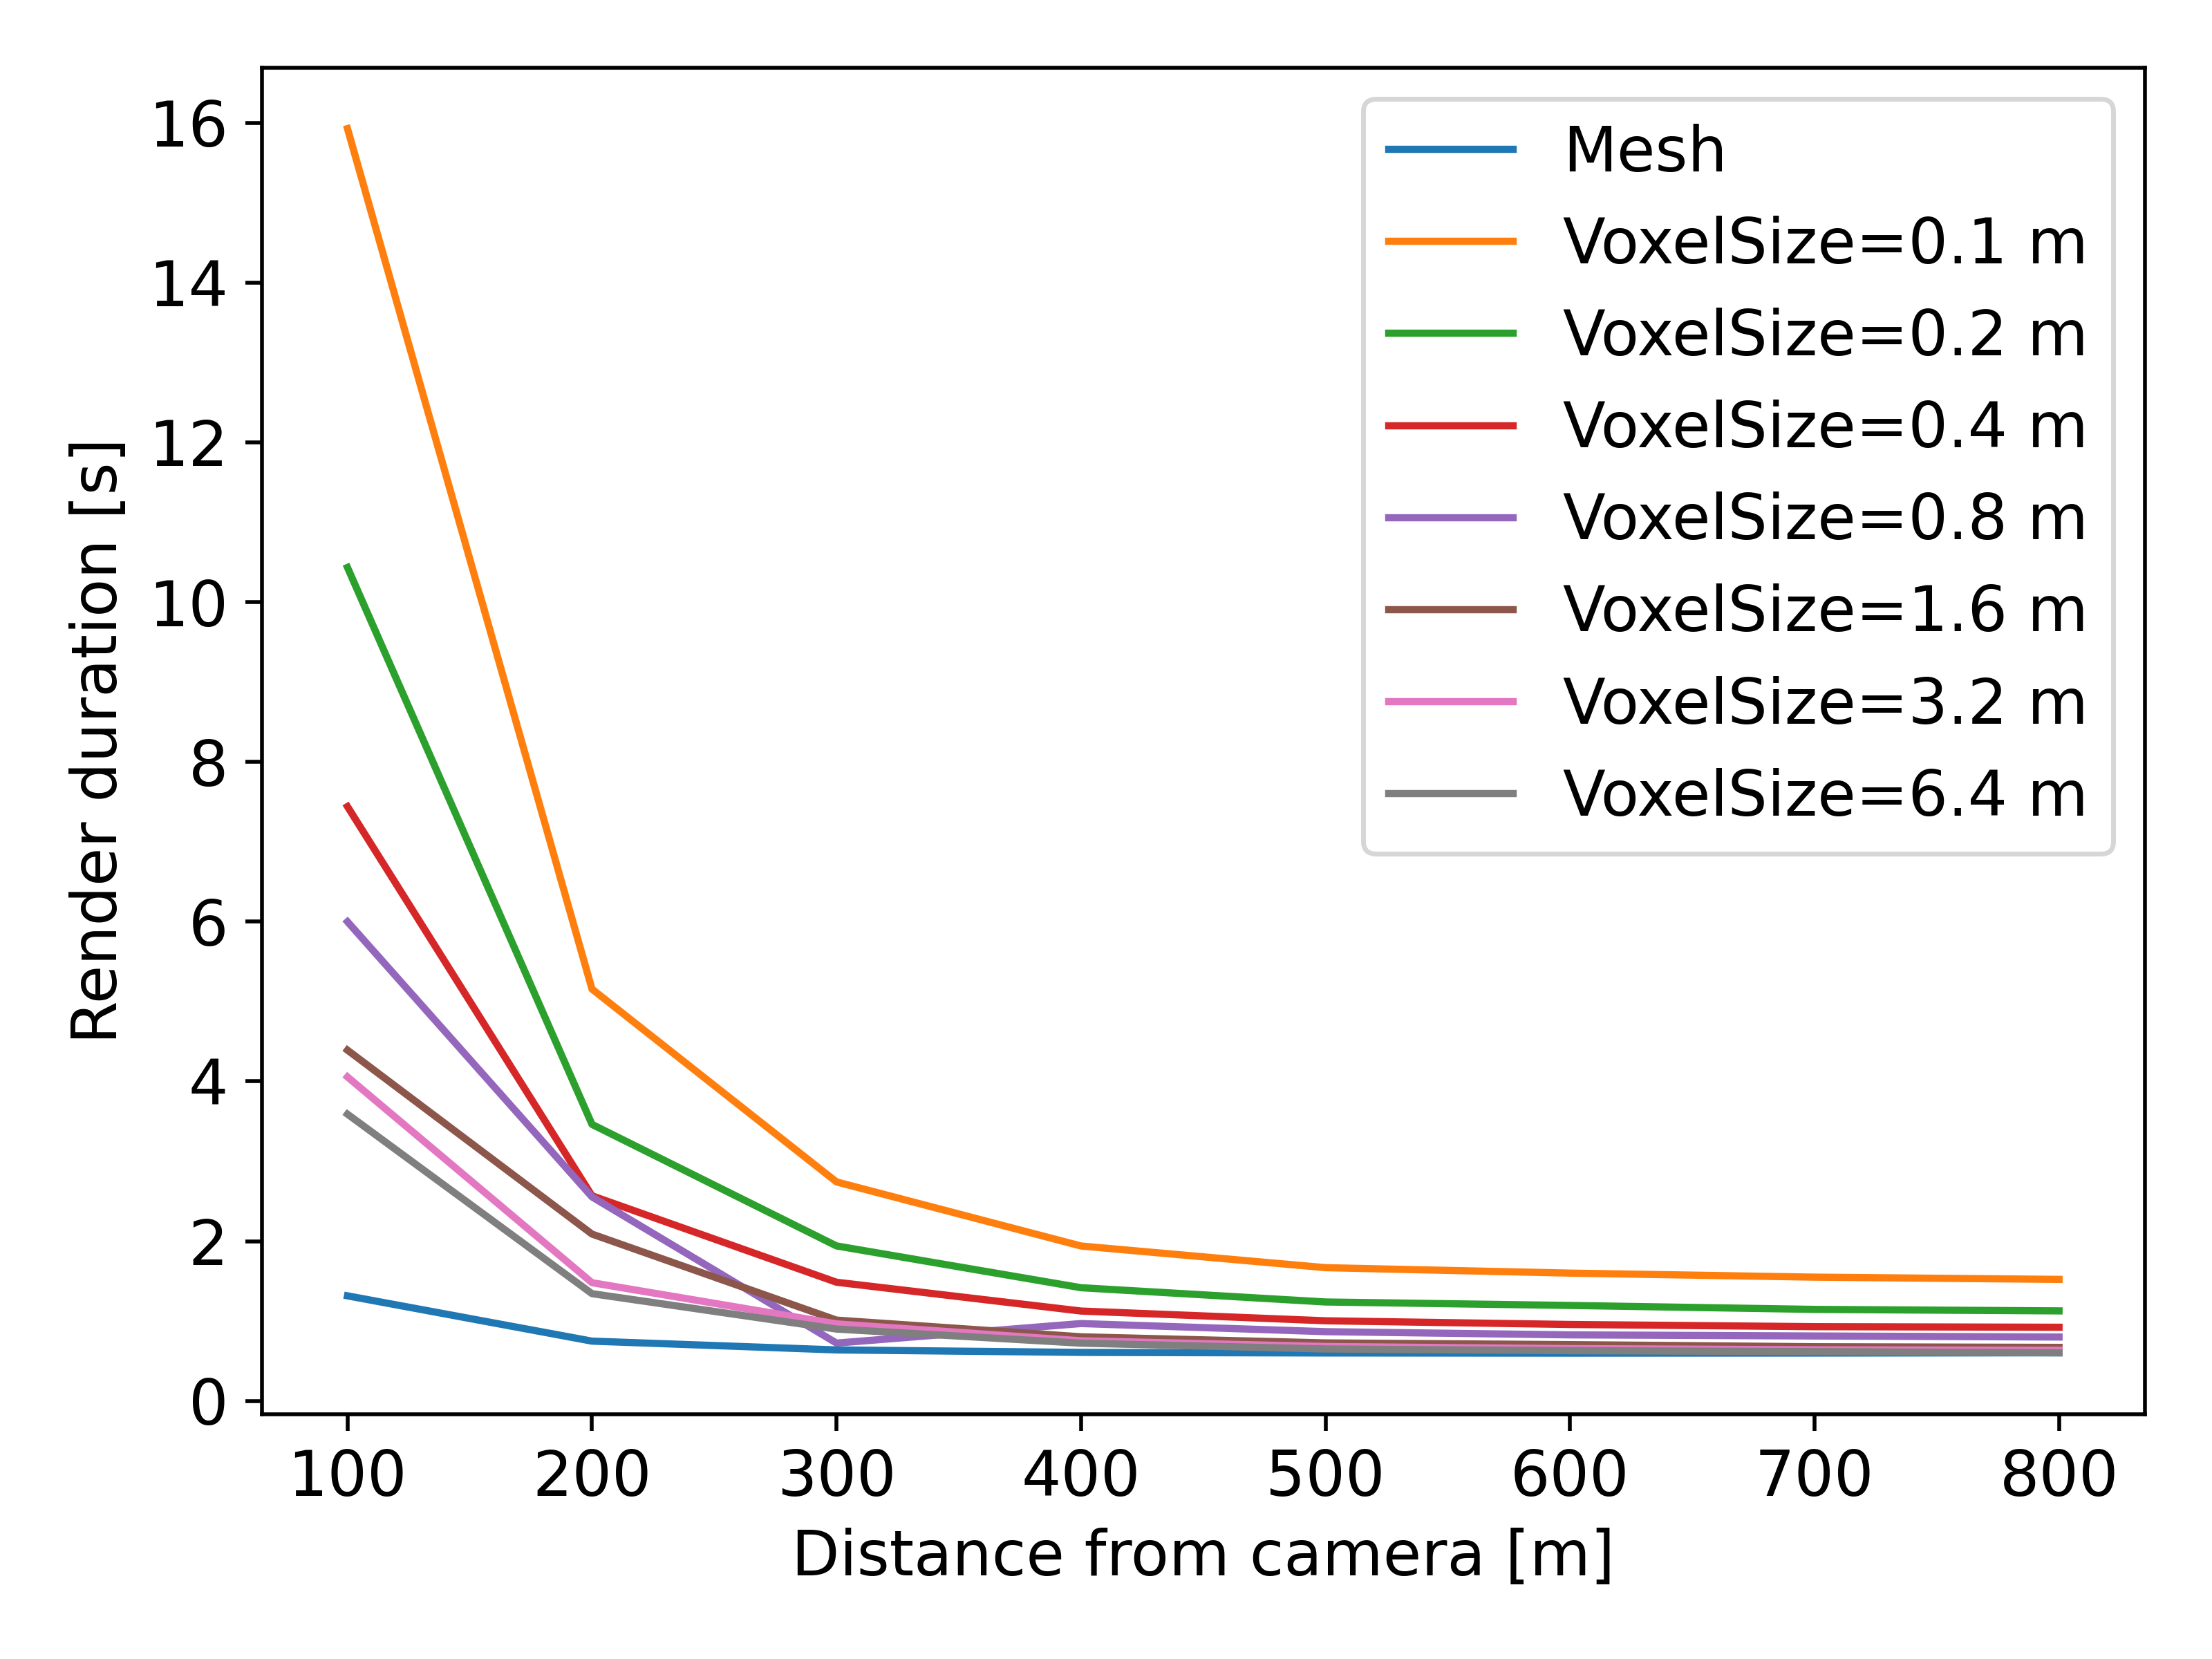
\includegraphics[width=1\linewidth]{img/results/render_durations_EU06a.png}
        \caption{}
    \end{subfigure}
    \begin{subfigure}[b]{0.49\linewidth}
        \centering
        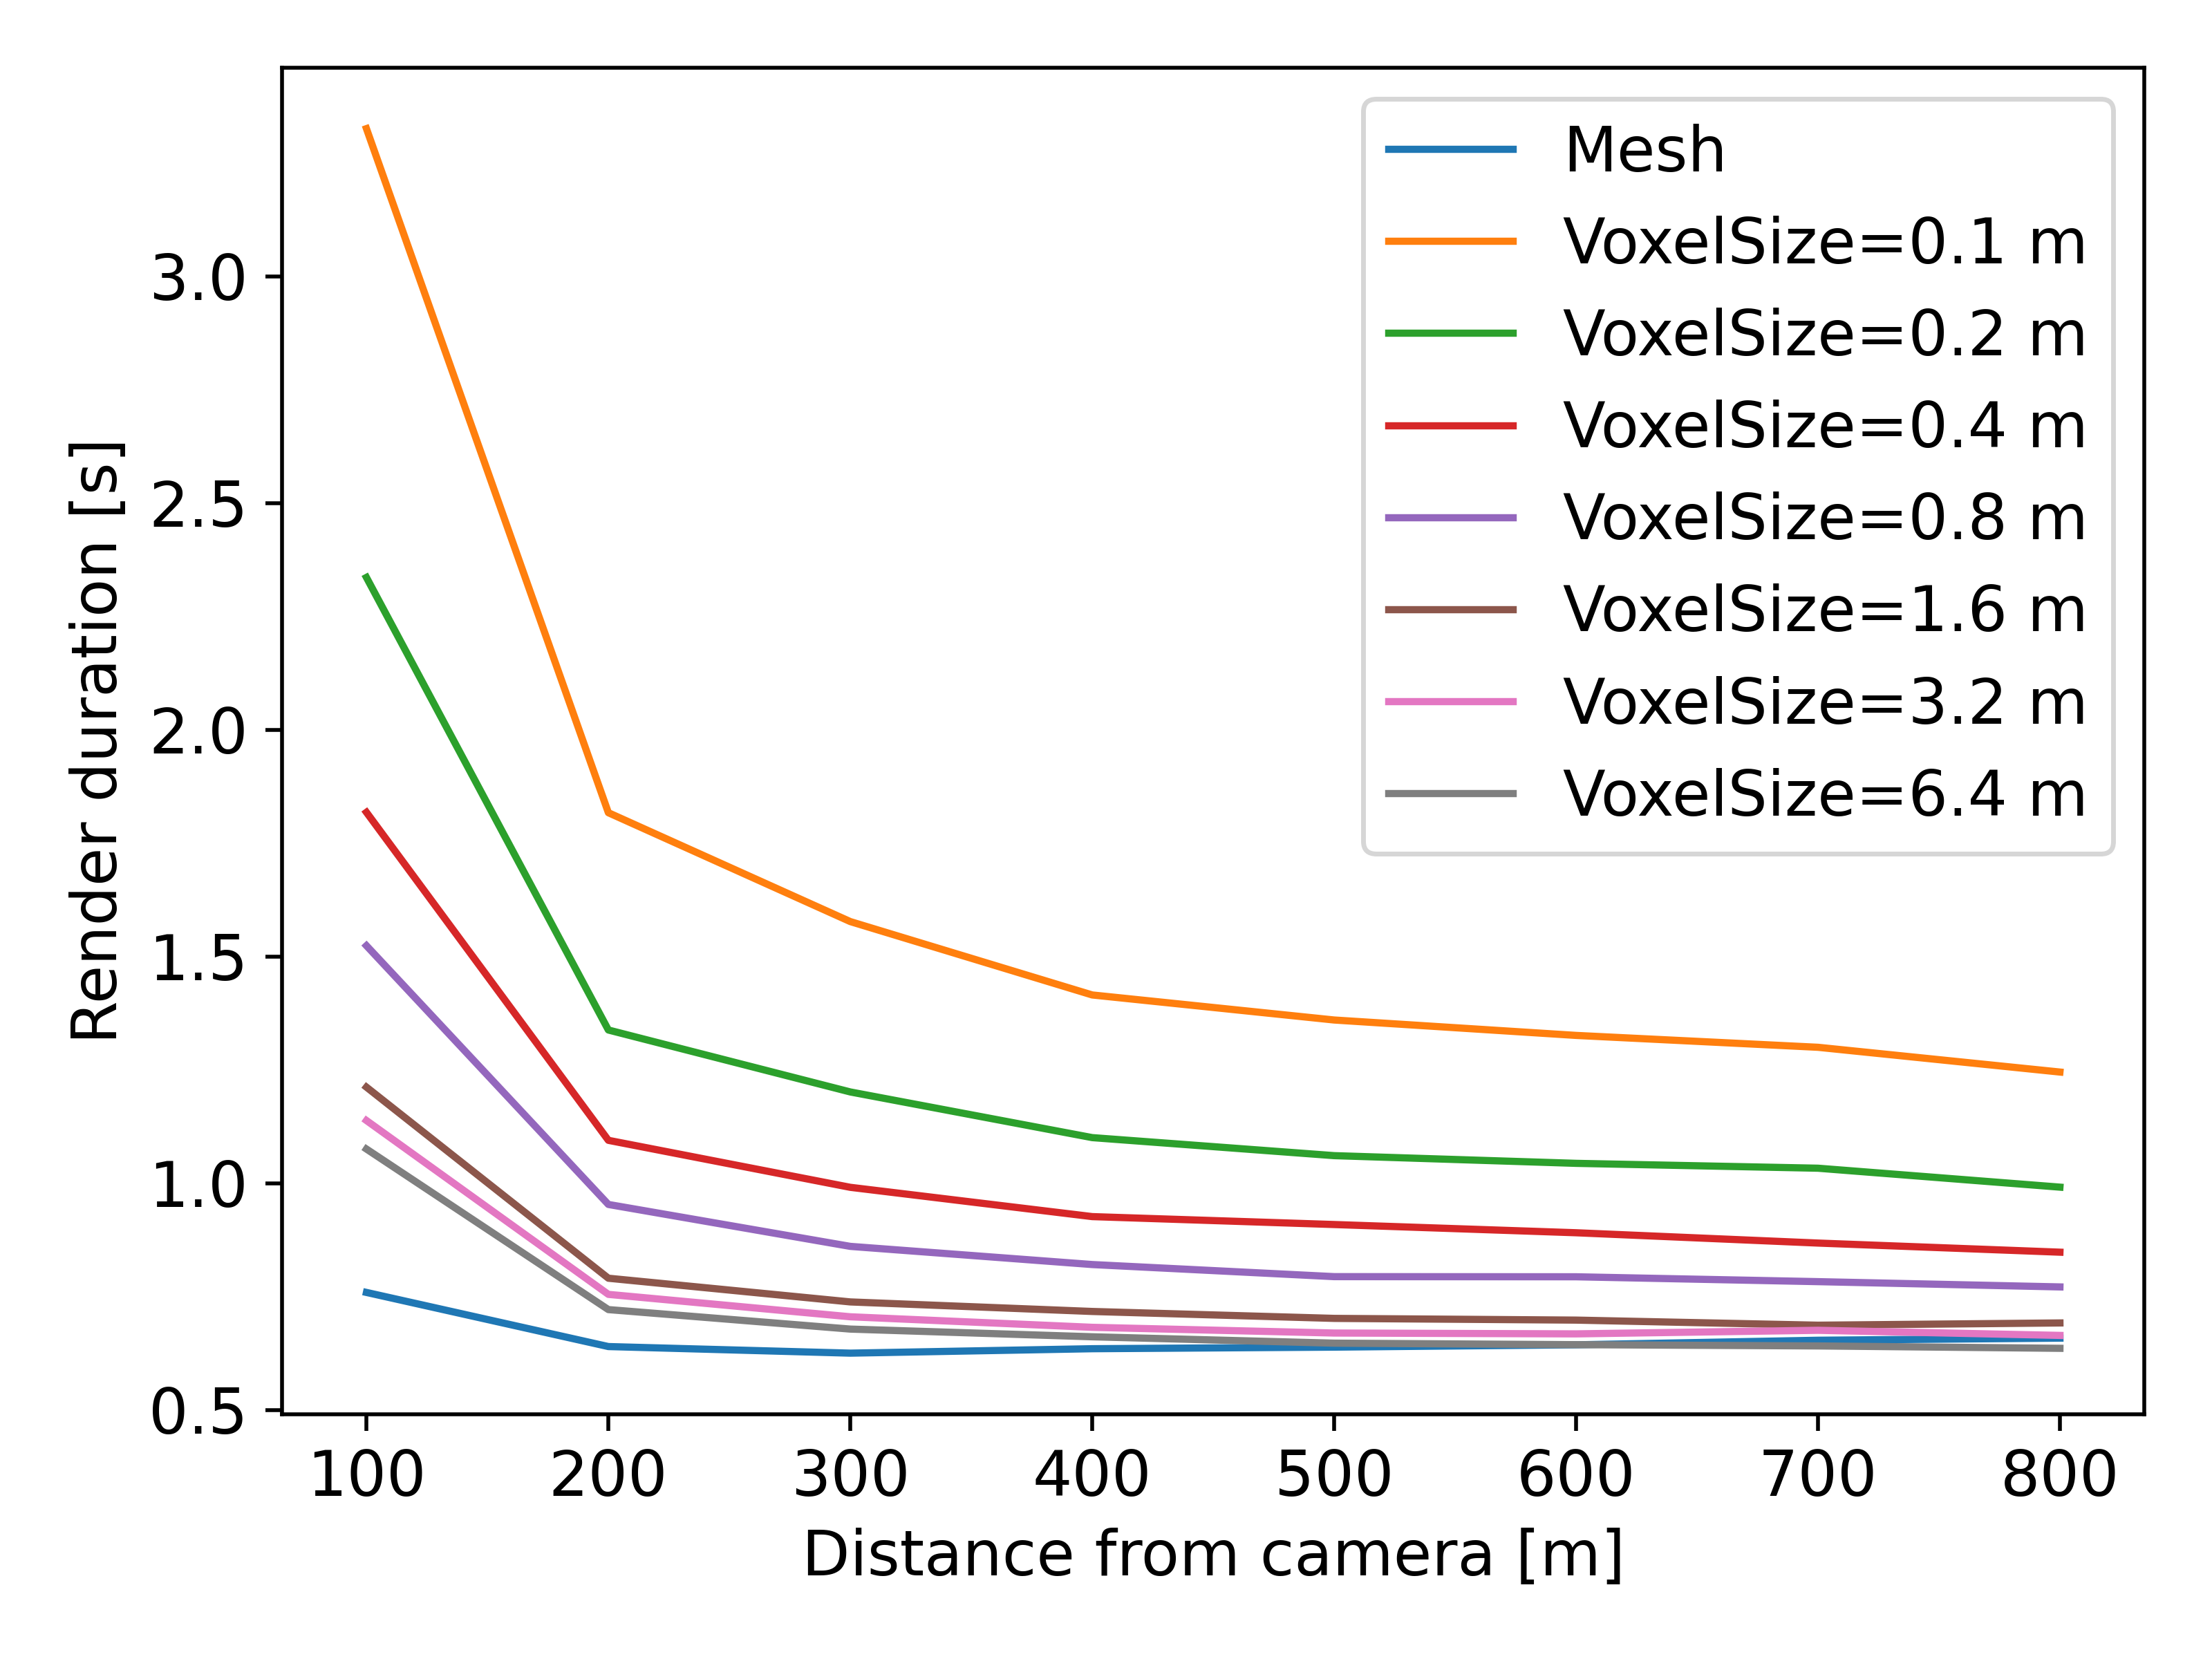
\includegraphics[width=1\linewidth]{img/results/render_durations_EA01a.png}
        \caption{}
    \end{subfigure}
	\caption[Plots of the render times depending on the distance from the camera]{These plots show the render times depending on the distance from the camera for single instances of the model \textit{Celtis australis adult} (a) and for \textit{Acer rubrum adult} (b). Meshes render faster than all \acsp{lod} until a certain distance.}
	\label{fig:render_time_comparisons}
\end{figure}
Interestingly, the meshes first render faster than all \acsp{lod}.
With increasing distance the rendertimes of the volumetric representations then decrease rapidly and eventually fall below the rendertime of the mesh representation.
For the model \textit{Celtis australis adult} this is the case after $\SI{800}{\m}$ and for the model \textit{Acer rubrum adult} a \ac{lod} renders faster after $\SI{700}{\m}$.
Surprisingly, the rendertimes for the mesh representations only decline in the beginning, but after a certain distance they rise steadily.
An explanation for this could be that at a certain distance the random sampling of a pixel produces large jumps across the bounding volume hierarchy, which leads to many cache misses.


As a second experiment we want to fix the distance between the camera and the model and measure how the image quality in terms of the \FLIP error and rendertimes change when we choose different \acsp{lod}.
Since the model covers only a small area of the image we crop the image before we compute the \FLIP error.
\begin{figure}[ht]
    \centering
    \begin{subfigure}[b]{0.49\linewidth}
        \centering
        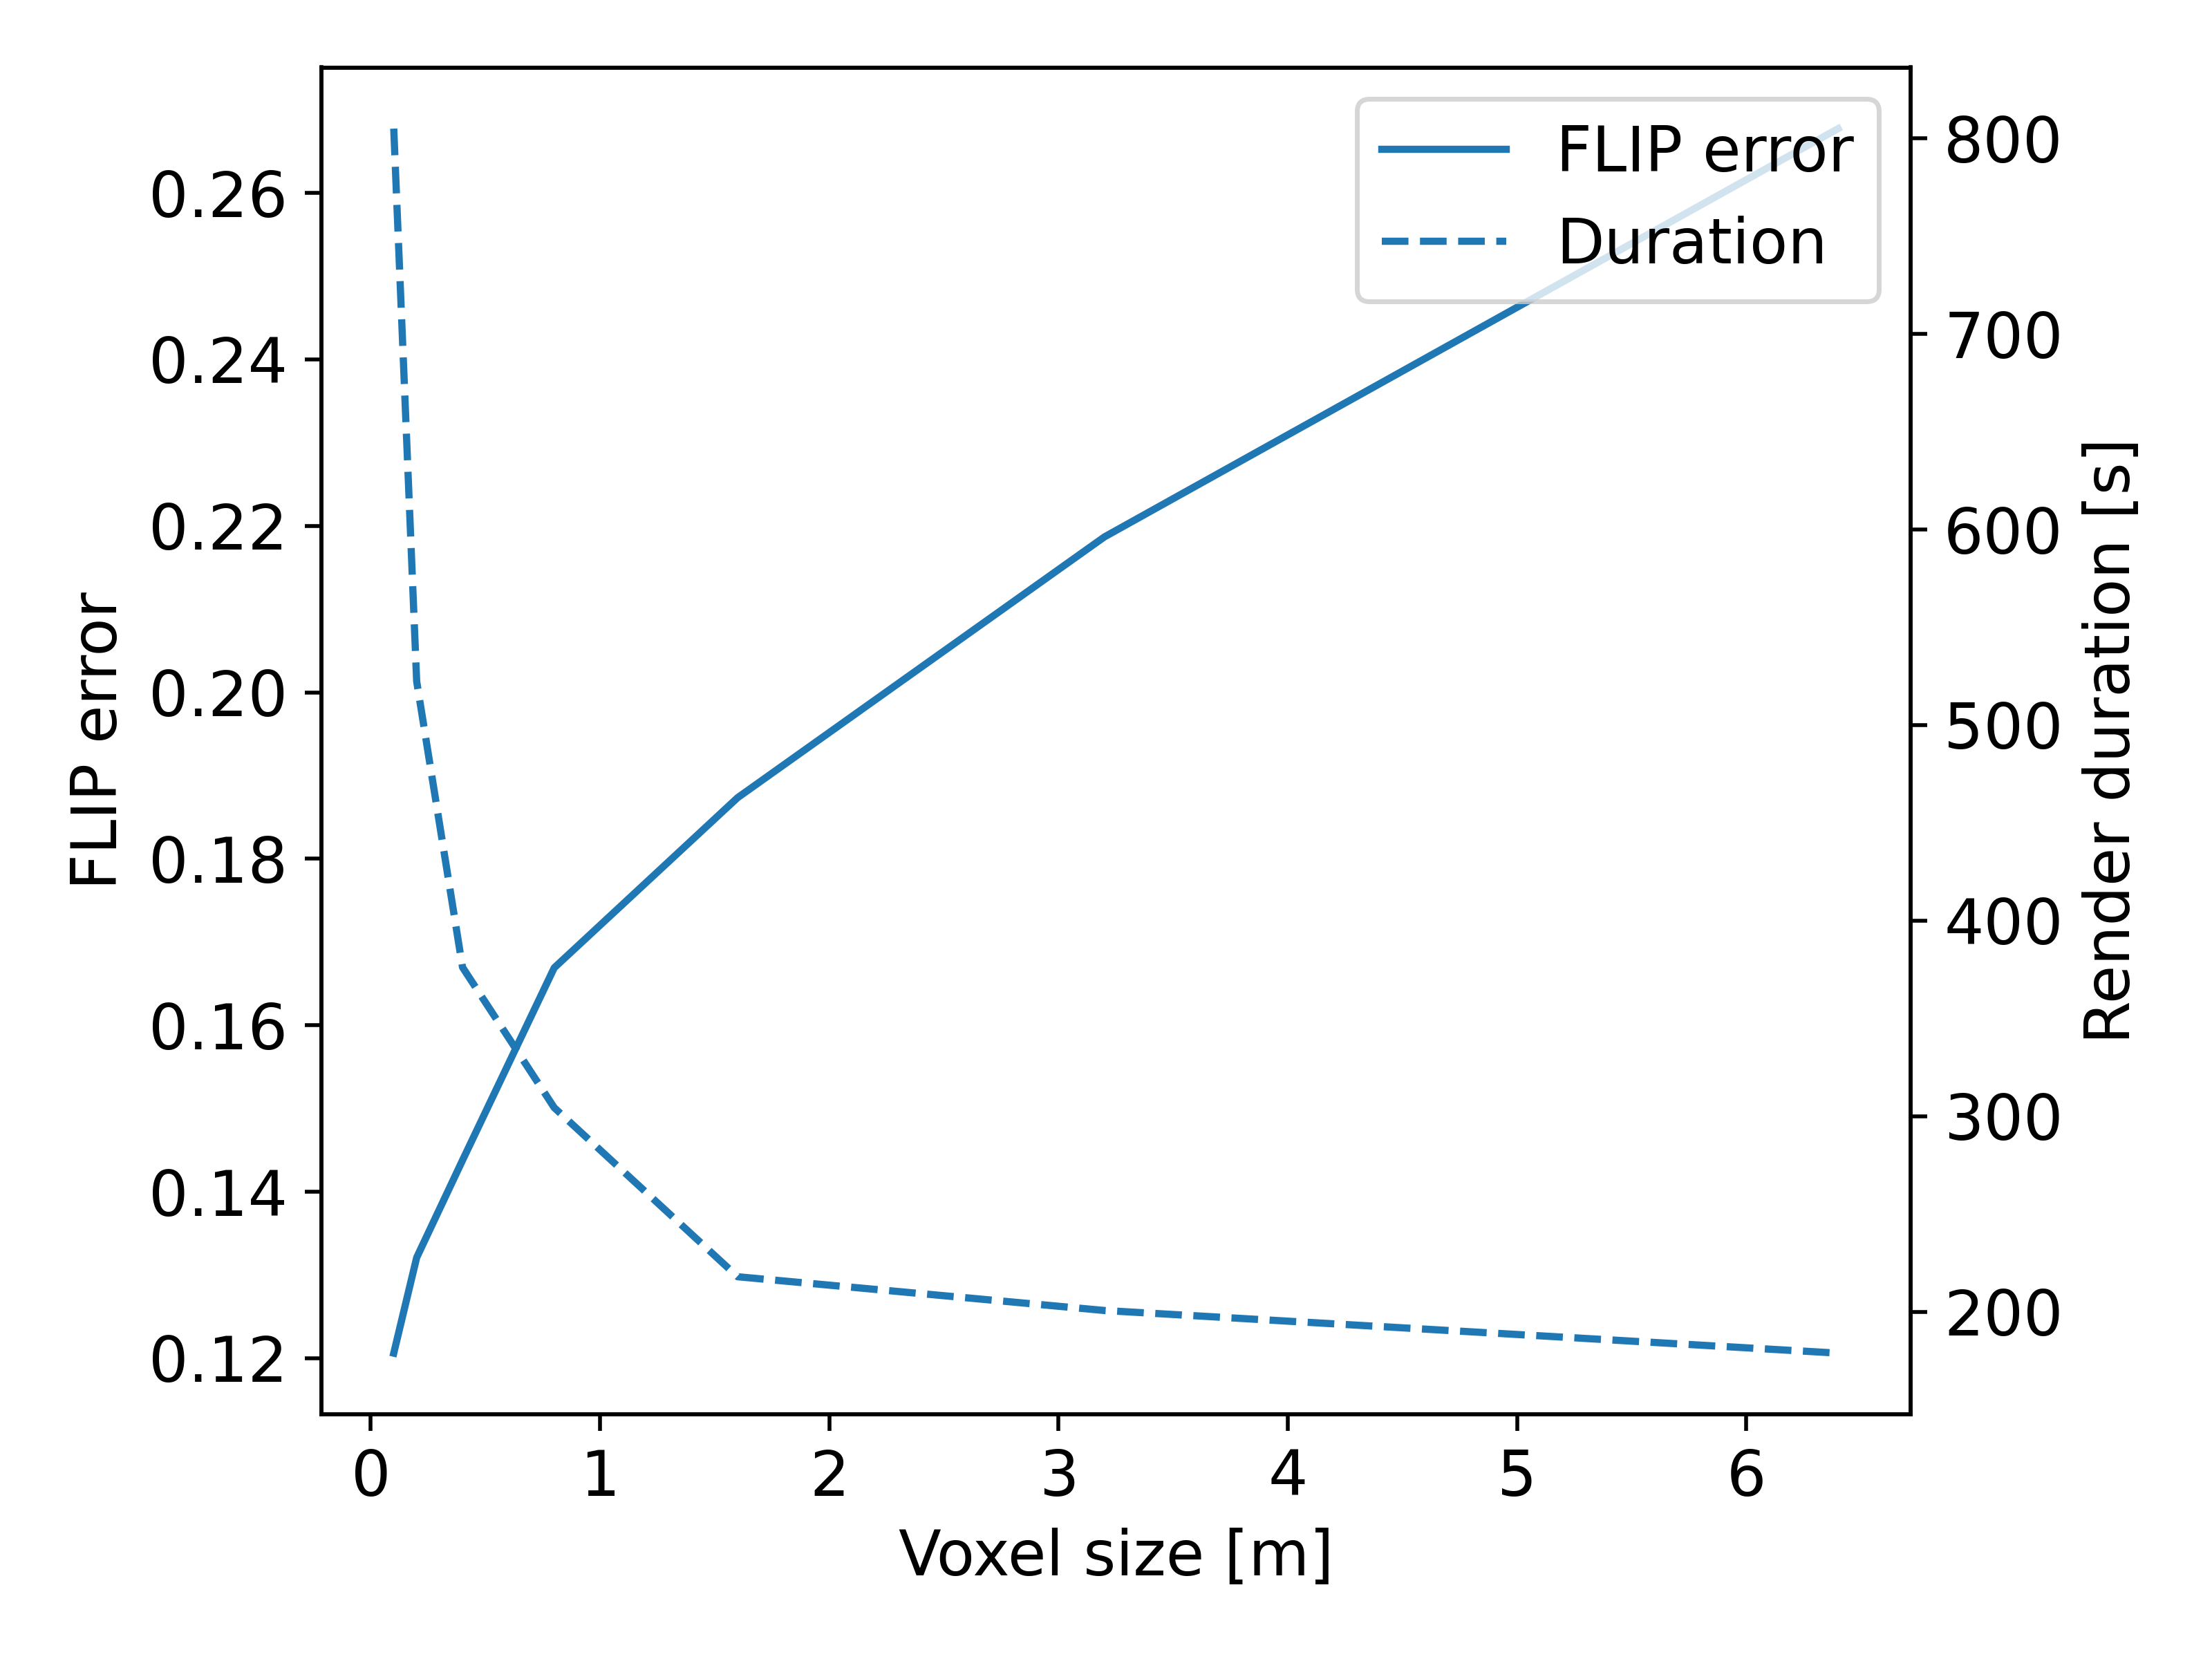
\includegraphics[width=1\linewidth]{img/results/performance_quality_EU06a.png}
        \caption{}
    \end{subfigure}
    \begin{subfigure}[b]{0.49\linewidth}
        \centering
        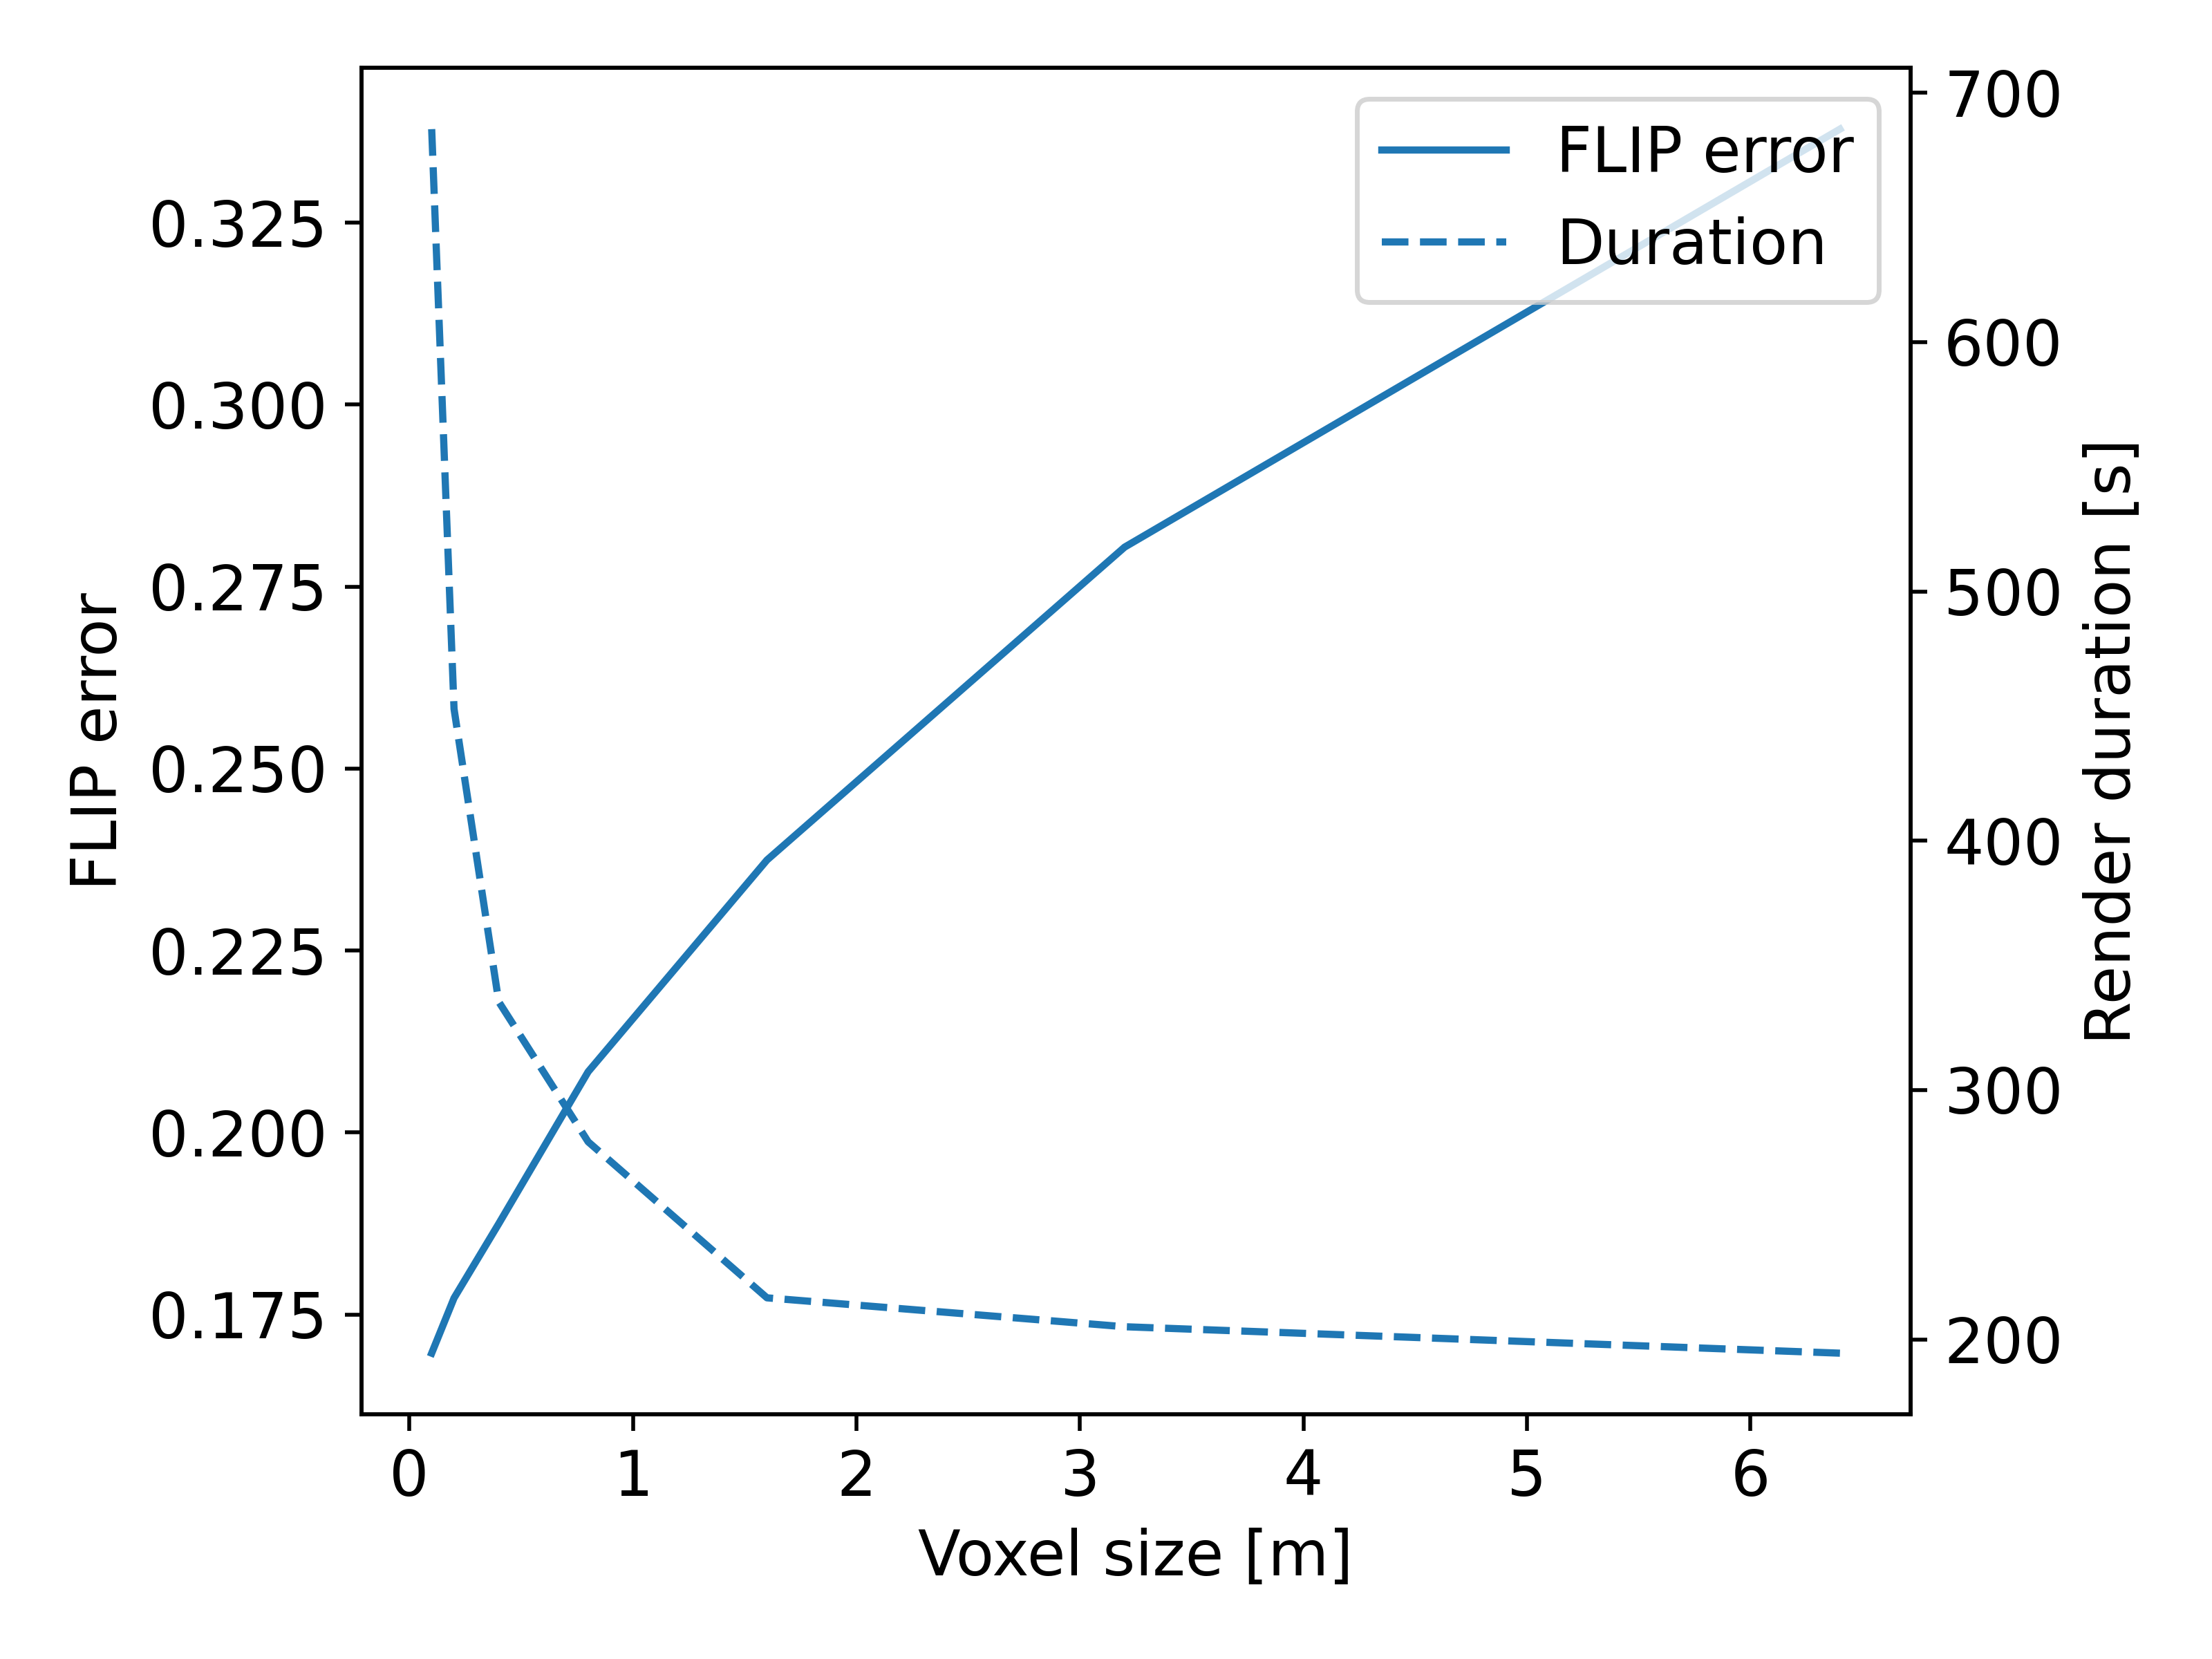
\includegraphics[width=1\linewidth]{img/results/performance_quality_EA01a.png}
        \caption{}
    \end{subfigure}
	\caption[Plots of \FLIP error and rendertimes for different \acsp{lod}]{These plots show the render times and mean \FLIP errors for different \acsp{lod}. (a) again shows the results for a single instance of the \textit{Celtis australis adult} model and (b) shows the results for \textit{Acer rubrum adult}. The \FLIP error is computed on a relevant image segment.}
	\label{fig:performance_quality}
\end{figure}
We observe in Figure \ref{fig:performance_quality} that the rendertimes fall in an exponential fashion, while the \FLIP errors show logarithmic growth.
Note however, that the voxel sizes of our \acsp{lod} increase exponentially by construction, which we have to consider in our interpretation.
We could alternatively draw the plots over the linear \ac{lod} level instead of the exponentially growing voxel size.
Regardless of the choice of the abscissa, the plots visualize the tradeoff really well that we have to make: We can either improve the performance by choosing rougher \acsp{lod} which leads to a high image error.
Or we aim for a high image quality by selecting a detailed \ac{lod}, which leads to longer rendertimes.
Another observation that we made during the single instance rendering is that the approach by \citeauthor{vicini2021non} of offsetting the scattered ray to the voxel border impairs the quality of the representation.
This is especially pronounced when rough \acsp{lod} are viewed from a close distance.






